\documentclass{article}

\usepackage[utf8]{inputenc}
\usepackage[italian]{babel}
\usepackage[T1]{fontenc}

\usepackage[a4paper,top=2cm,bottom=2cm,left=3cm,right=3cm]{geometry}\usepackage{nameref,zref-xr}
%\usepackage{xr-hyper}
\usepackage{hyperref, amsmath, amssymb, graphicx, mathtools, xcolor, enumitem, verbatim, todonotes, csquotes, subcaption, fancyhdr, lastpage, cancel, xspace, float, caption, prettyref, tabularx, colortbl, color, soul, listings, caption}
\usepackage[most]{tcolorbox}
%\usepackage[inkscapeformat=png, inkscapelatex=false, inkscapearea=page]{svg}
\usepackage[inkscapelatex=false, inkscapearea=page]{svg}
\usepackage[bottom]{footmisc}

\zxrsetup{toltxlabel} % allows to use the \ref command as usual

\definecolor{viola}{rgb}{0.4157, 0.698, 0.7922}


%Link per il D1

%\externaldocument[D1-]{../D1/out/ObiettiviDelProgetto}[D1.pdf]
\zexternaldocument*[D1-]{../D1/out/ObiettiviDelProgetto}
\newrefformat{D1-ob}{\color{cyan}D1 \ref{#1}\color{black} }

%\externaldocument[D1-]{../D1/out/RequisitiFunzionali}[D1.pdf]
\zexternaldocument*[D1-]{../D1/out/RequisitiFunzionali}
\newrefformat{D1-rf}{\color{cyan}D1 \ref{#1}\color{black} }

%\externaldocument[D1-]{../D1/out/RequisitiNonFunzionali}[D1.pdf]
\zexternaldocument*[D1-]{../D1/out/RequisitiNonFunzionali}
\newrefformat{D1-rnf}{\color{cyan}D1 \ref{#1}\color{black} }

%\externaldocument[D1-]{../D1/out/RequisitiFrontEnd}[D1.pdf]
\zexternaldocument*[D1-]{../D1/out/RequisitiFrontEnd}
\newrefformat{D1-fe}{\color{cyan}D1 \ref{#1}\color{black} }

%\externaldocument[D1-]{../D1/out/RequisitiBackEnd}[D1.pdf]
\zexternaldocument*[D1-]{../D1/out/RequisitiBackEnd}
\newrefformat{D1-be}{\color{cyan}D1 \ref{#1}\color{black} }


%Link per il D2

%\externaldocument[D2-]{../D2/out/AnalisiDeiComponenti}[D2.pdf]
\zexternaldocument*[D2-]{../D2/out/AnalisiDeiComponenti}
\newrefformat{D2-aci}{\color{cyan}D2 \ref{#1}\color{black} }
\newrefformat{D2-dci}{\color{cyan}D2 \ref{#1}\color{black} }

%\externaldocument[D2-]{../D2/out/AnalisiDelContesto}[D2.pdf]
\zexternaldocument*[D2-]{../D2/out/AnalisiDelContesto}
\newrefformat{D2-aco}{\color{cyan}D2 \ref{#1}\color{black} }
\newrefformat{D2-dco}{\color{cyan}D2 \ref{#1}\color{black} }

%\externaldocument[D2-]{../D2/out/RequisitiFunzionali}[D2.pdf]
\zexternaldocument*[D2-]{../D2/out/RequisitiFunzionali}
\newrefformat{D2-uc}{\color{cyan}D2 \ref{#1}\color{black} }

%\externaldocument[D2-]{../D2/out/RequisitiNonFunzionali}[D2.pdf]
\zexternaldocument*[D2-]{../D2/out/RequisitiNonFunzionali}
\newrefformat{D2-rnfd2}{\color{cyan}D2 \ref{#1}\color{black} }


%Link per il D3

%\externaldocument[D3-]{../D3/out/DiagrammaDelleClassi}[D3.pdf]
\zexternaldocument*[D3-]{../D3/out/DiagrammaDelleClassi}
\newrefformat{D3-dcl}{\color{cyan}D3 \ref{#1}\color{black} }

%\externaldocument[D3-]{../D3/out/ObjectConstraintLanguage}[D3.pdf]
\zexternaldocument*[D3-]{../D3/out/ObjectConstraintLanguage}
\newrefformat{D3-ocl}{\color{cyan}D3 \ref{#1}\color{black} }

%\externaldocument[D3-]{../D3/out/DiagrammaECodiceObjectConstraintLanguage}[D3.pdf]
\zexternaldocument*[D3-]{../D3/out/DiagrammaECodiceObjectConstraintLanguage}
%\newrefformat{D3-uc}{\color{cyan}D3 \ref{#1}\color{black}}


\title{Documento di progetto}
\author{Gruppo T56}
\date{A.A. 2022-2023}

%\setlength\parindent{0pt}

\setcounter{tocdepth}{5}
\setcounter{secnumdepth}{5}

\lhead{\textbf{Document: }Documento di progetto}
\rhead{\textbf{Revision: }0.1}
\cfoot{\thepage /\pageref{LastPage}}

\hypersetup{
    colorlinks=true,
    linkcolor=blue,
    urlcolor=blue,
    pdftitle={Documento di progetto - T56},
}

\pagestyle{fancy}
\newcommand{\nome}[0]{Life Planner}

\begin{document}

\begin{titlepage}
    \begin{figure}[!htb]
        \minipage{0.5\textwidth}
        
\includegraphics[width=0.7\textwidth]{img/logo_unitn.png}
        \endminipage
        \hfill
        \minipage{0.5\textwidth}
        \begin{flushright}
            \Large
            Dipartimento d'Ingegneria e Scienze dell'informazione
        \end{flushright}
        \endminipage
        \hfill
    \end{figure}

    \vspace{3cm}

    \large
    \textbf{Progetto:}
    \begin{center}
        \Huge
        \color{blue}
        \textbf{\nome}
    \end{center}

    \vspace{1cm}

    \textbf{Titolo del documento:}
    \begin{center}
        \huge
        \color{blue}
        \textbf{Documento di progetto}\\
        \textbf{(Obiettivi, Requisiti, Design Front-End e Back-End)}
    \end{center}

    \vspace{2cm}

    \begin{center}
        
\includegraphics[width=0.7\textwidth, height=0.2\textheight]{img/LogoNuovo.png}
    \end{center}
    \vspace{2cm}

    \begin{center}
        \large
        \textbf{Gruppo T56}\\
        \textbf{Gabriele Lacchin, Denis Lucietto ed Emanuele Zini}
    \end{center}

\end{titlepage}
\pagebreak

\tableofcontents
\pagebreak

\section*{Scopo del documento}
\addcontentsline{toc}{section}{Scopo del documento}
Lo scopo di questo documento è presentare gli obiettivi e i requisiti del progetto \nome ideato da Gabriele Lacchin, Denis Lucietto ed Emanuele Zini.\\
Il seguente documento presenta:
\begin{itemize}
    \item \hyperref[sec:ObiettiviProgetto]{gli obiettivi del sistema};
    \item \hyperref[sec:RequisitiFunzionali]{i requisiti funzionali};
    \item \hyperref[sec:RequisitiNonFunzionali]{i requisti non funzionali};
    \item \hyperref[sec:RequisitiFrontEnd]{i requisiti di Front-End};
    \item \hyperref[sec:RequisitiBackEnd]{i requisiti del Back-End}.
\end{itemize}
\section{Obiettivi del progetto}
\label{sec:ObiettiviProgetto}
Il progetto ha come obiettivo la realizzazione di un calendario automatizzato.\\
Il sito si pone come un sistema automatizzato di programmazione del tempo in base agli impegni che si inseriscono, avendo la possibilità d'imporre delle preferenze per la disposizione delle attività da svolgere.\\
La funzione principale della piattaforma è la facilitazione del processo di programmazione del proprio tempo.

\vspace{0.5cm}

Nello specifico questa applicazione permette di:
\begin{listaPersonale}{OB}
      \elemento {ob:1} registrarsi al sito e autenticarsi con servizi di terzi parti, in modo tale da semplificare la registrazione e futuri accessi da parte dell'utente e di permettere agli utenti non registrati di accedere ad alcune funzionalità della piattaforma;
      \elemento {ob:2} aggiungere eventi al calendario e poterli gestire in modo tale da personalizzarli secondo le proprie preferenze;
      \elemento {ob:3} formattare automaticamente il calendario in base agli impegni e ai ritardi così da ottenere delle giornate sempre organizzate;
      \elemento {ob:4} avere notifiche per ciascun impegno avendo la possibilità di personalizzarle in base alle proprie preferenze;
      \elemento {ob:5} interagire con servizi di terze parti per aumentare le funzionalità offerte dalla piattaforma ed essere adattabile a dispositivi di dimensione variabile;
      \elemento {ob:6} avere accesso a funzioni premium e gestirne il pagamento in modo da offrire più funzionalità e rendere il servizio offerto economicamente sostenibile;
      \elemento {ob:7} ottenere un resoconto a fine giornata delle attività;
      \elemento {ob:8} gestire più calendari e interagire con calendari di altri utenti per poter organizzare attività in comune;
      \elemento {ob:9} interagire con l'applicativo in modo sicuro in modo tale che eventuali attacchi di rete non permettano di carpire alcuna informazione privata dell'utente; inoltre il sito deve garantire l'adempimento delle leggi sulla privacy presenti nel GDPR dell'Unione europea;
      \elemento {ob:10} filtrare gli impegni in base a dei criteri di ricerca;
      \elemento {ob:11} avere una web app in modo tale da estendere le funzionalità e portabilità del sito;
      \elemento {ob:12} ottenere informazioni sull'uso del tempo così da tenere gli utenti aggiornati sulle giornate;
      \elemento {ob:13} avere un qualsiasi numero di utenti attivi nel sito contemporaneamente;
      \elemento {ob:14} avere un sito affidabile, prestante, compatibile con diversi browser e che sia in italiano;
\end{listaPersonale}

\section{Requisiti funzionali}
\label{sec:RequisitiFunzionali}

Nel seguente capitolo verranno presentati i requisiti funzionali (RF) del sistema con la motivazione della loro presenza e legame con gli obiettivi sopra citati.

\begin{listaPersonale}{RF}
	\elemento[ACCESSO E REGISTRAZIONE AL SITO]{rf:1} Il sistema deve permettere all'utente di avere 3 livelli di accesso:
	\begin{itemize}
		\item utente autenticato-standard(\ref{ob:1});
		\item utente non autenticato (\ref{ob:1});
		\item utente autenticato-premium (\ref{ob:6});
	\end{itemize}
	Il sistema deve permettere all'utente di registrarsi sul sito (\ref{ob:1}) in qualsiasi momento esso voglia, seguendo le regole definite in RNF\ref{rnf:2.1}; inoltre, la piattaforma deve permettere di abbonarsi al servizio premium, con un account preesistente o durante la fase di registrazione.\\
	A ogni modo il sistema deve rendere disponibile all'utente di utilizzare la piattaforma anche come utente non autenticato in versione demo(\ref{rf:3}) cosicché possa provare il sito prima di registrarsi.

	\begin{listaPersonale2}{RF}
		\elemento[METODI AUTENTICAZIONE]{rf:1.1} L'autenticazione può essere fatta con email e password o con servizi di terze parti, più nello specifico con Google. (\ref{ob:1}).
	\end{listaPersonale2}

	\elemento[UTENTE AUTENTICATO-STANDARD]{rf:2} Un utente autenticato standard è un utente registrato che ha effettuato il login e che usufruisce delle funzionalità base della piattaforma.

	\begin{listaPersonale2}{RF}
		\elemento[FUNZIONALITA']{rf:2.1} Il sistema offrirà agli utenti con account autenticato-standard tutti i servizi sottoelencati, eccetto quelli descritti nella sezione utente autenticato-premium (\ref{rf:2.2}), con le limitazioni elencate in \ref{rf:2.2.2}. Inoltre sarà possibile aggiungere o modificare il proprio username da usare per un più rapido riconoscimento nei calendari condivisi.

		\elemento[UTENTE AUTENTICATO-PREMIUM]{rf:2.2} L'utente avrà la possibilità anche di accedere a un maggior numero di funzionalità della piattaforma grazie alla sottoscrizione di un abbonamento mediante un pagamento mensile(\ref{ob:6}). Inoltre il pagamento degli utenti premium contribuirà alla sostenibilità economica del sito.

		\begin{listaPersonale3}{RF}
			\elemento[PAGAMENTO]{rf:2.2.1} Il sistema offrirà la possibilità all'utente di pagare l'abbonamento con un servizio di pagamento esterno. (\ref{ob:6})

			\elemento[FUNZIONALITA' AGGIUNTIVE(\ref{ob:6})]{rf:2.2.2} Grazie all'account premium, il sistema permetterà di accedere alle funzionalità standard e a dei servizi aggiuntivi:
			\begin{itemize}
				\item poter avere un numero illimitato di calendari personali in base allo loro scopo: gli utenti non premium potranno avere solo 5 calendari personali (\ref{rf:4.2}).
				\item poter avere un numero illimitato di calendari condivisi: gli utenti standard potranno averne 3 (\ref{rf:4.1}).
			\end{itemize}

		\end{listaPersonale3}
	\end{listaPersonale2}

	\elemento[UTENTE NON AUTENTICATO]{rf:3} Nel caso di un utente non autenticato (\ref{ob:1}), il sistema permetterà di effettuare l'accesso e/o registrazione nelle modalità descritte in \ref{rf:1}. Nel caso l'utente non volesse registrarsi, il sito darà la possibilità di usufruire delle funzionalità in versione demo.

	\begin{listaPersonale2}{RF}
		\elemento[DEMO]{rf:3.1}	L'utente non autenticato avrà la possibilità di utilizzare il sito senza che le modifiche fatte vengano salvate sui server della piattaforma; nel caso in cui l'utente si registrasse sul sito, verranno caricate e rese disponibili su più dispositivi.

		\begin{listaPersonale3}{}
			\elemento[FUNZIONALITÀ MANCANTI]{rf:3.1.1} L'utente non autenticato non avrà a disposizione diverse funzionalità tra cui \ref{rf:4}, \ref{rf:8}, \ref{rf:10}, \ref{rf:11}, \ref{rf:14} e \ref{rf:15}.
		\end{listaPersonale3}
	\end{listaPersonale2}

	\elemento[CONDIVISIONE DEL CALENDARIO]{rf:4} Il sistema darà la possibilità di condividere il proprio calendario su più dispositivi (\ref{ob:8}).

	\begin{listaPersonale2}{RF}
		\elemento[INTERAZIONE DI CALENDARI CON ALTRE PERSONE]{rf:4.1} Il sistema deve offrire la possibilità agli utenti autenticati d'interagire tra loro mediante la condivisione e integrazione dei loro calendari (\ref{ob:8}). Grazie alla condivisione e integrazione dei calendari tra gli utenti del sito, i clienti avranno la possibilità di programmare gli eventi in comune.
		\elemento [CALENDARI PERSONALI] {rf:4.2} La piattaforma deve rendere possibile all’utente di avere più calendari personali (\ref{ob:8}) riguardo alle varie attività da svolgere, che si possono visualizzare ogni qualvolta si voglia. Il numero di calendari personali, reso disponibile dal sito, dipende dal tipo di account dell’utente (\ref{rf:2.2.2}).
	\end{listaPersonale2}

	\elemento[CREAZIONE/MODIFICA EVENTO]{rf:5} Il sistema deve dare la possibilità all'utente di aggiungere, eliminare e modificare un evento del calendario mediante l'utilizzo di un pop-up (\ref{ob:2}) e nella schermata dedicata agli eventi. Nella compilazione dell'attività, il sistema deve permettere al cliente:
	\begin{listaPersonale2}{}
		\elemento{rf:5.1} d'imporre restrizioni, ovvero definire ora e giorno dell'attività da svolgere o define una scadenza,deadline;
		\elemento{rf:5.2} impostare la priorità dell'impegno;
		\elemento{rf:5.3} scrivere una descrizione e un titolo;
		\elemento{rf:5.4} definire impegni di routine oppure impegni ripetuti su più giorni, chiamate "Abitudini".
		\elemento{rf:5.5} aggiungere il luogo dove si terrà l'impegno;
		\elemento{rf:5.6} condividere l'evento con altri utenti;
		\elemento {rf:5.7} di poter aggiungere l'evento ad un raggruppamento di altre attività; un raggruppamento è un insieme di attività presenti nel calendario principale;
		\elemento {rf:5.8} impostare la difficoltà, ovvero definire la complessità dell'evento da completare;
		\elemento{rf:5.9} impostare notifiche come descritto in \ref{rf:7}.
	\end{listaPersonale2}


	\elemento[INSERIMENTO IMPEGNO]{rf:6} Una volta compilato il pop-up di aggiunta impegno, il sistema deve inserire automaticamente l'impegno nel calendario (\ref{ob:3}) seguendo le restrizioni, difficoltà, priorità e gli altri campi inseriti dall'utente a tempo di compilazione dell'evento (\ref{rf:5}).

	\elemento[NOTIFICHE]{rf:7} Il sistema deve inviare delle notifiche per ciascun impegno (\ref{ob:4}), fornendo la possibilità di personalizzarle, infatti nel pop-up di compilazione dell'evento (\ref{rf:5}) deve essere possibile:
	\begin{listaPersonale2}{}
		\elemento{rf:7.1} impostare quando ricevere tale notifica
		\elemento{rf:7.2} definire il titolo della notifica: di default quest'ultimo sarà il titolo dell'evento.
	\end{listaPersonale2}

	\elemento[INTERAZIONE CON SISTEMI DI TERZE PARTI]{rf:8} Il sito deve permettere all'utente d'interagire con sistemi di terzi parti (\ref{ob:5}), ad esempio:

	\begin{listaPersonale2}{RF}
		\elemento[INTERAZIONE con GOOGLE CALENDAR]{rf:8.1} In quanto è un'applicazione molto diffusa tra gli utenti che utilizzano calendari, il sistema deve rendere possibile all'utente di poter interagire con eventi di Google Calendar. In particolare la piattaforma deve permettere di:
		\begin{listaPersonale3}{}
			\elemento{rf:8.1.1} importare ed esportare manualmente;
			\elemento{rf:8.1.2} importare ed esportare in automatico.
		\end{listaPersonale3}

		\elemento[INTERAZIONE CON UN SERVIZIO DI MAPPE]{rf:8.2} Il sistema darà la possibilità all'utente di aggiungere il luogo dove si svolgerà l'impegno.
	\end{listaPersonale2}

	\elemento[INFORMAZIONI sull'USO del TEMPO]{rf:9} Il sito deve presentare delle infografiche e liste riguardanti l'utilizzo del tempo. L'utente, così, potrà visualizzare dei grafici esemplificativi su come viene speso il proprio tempo. (\ref{ob:12})

	\elemento[RIORGANIZZAZIONE DI ATTIVITA']{rf:10} Il sistema deve riorganizzare automaticamente il calendario in caso di ritardi (\ref{ob:3}). Sarà data la possibilità all'utente di notificare il sistema di ritardi e il sito dovrà ripianificare il calendario, sempre secondo le regole descritte nel \ref{rf:6}.

	\elemento[RESOCONTO GIORNATA]{rf:11} Il sistema, a fine giornata, deve presentare un resoconto (\ref{ob:7}), dove l'utente potrà comunicare le attività fatte e non, in modo tale da dare la possibilità al sistema di ricalcolare eventuali modifiche in base agli impegni non conclusi sempre secondo le modalità citate in \ref{rf:6}.

	\elemento[FILTRO IMPEGNI]{rf:12} Il sito offrirà la possibilità di poter visualizzare gli impegni dato un specifico filtro(\ref{ob:10}) definito dall'utente secondo alcuni criteri:
	\begin{listaPersonale2}{}
		\elemento{rf:12.1} titolo evento con corrispondenza totale o parziale;
		\elemento{rf:12.2} data evento;
		\elemento{rf:12.3} priorità evento;
		\elemento{rf:12.4} persone incluse nell'evento.
	\end{listaPersonale2}

	\elemento[IMPOSTAZIONI PREDEFINITE DI UN CALENDARIO]{rf:13} Ogni calendario avrà una sezione dedicata dove l'utente potrà modificare le impostazioni predefinite del calendario(\ref{ob:8}). Queste impostazioni saranno usate per precompilare i campi dell'evento, che si sta aggiungendo. L'utente, durante la fase di aggiunta dell'evento, potrà modificare i campi precompilati(\ref{ob:2}). La sezione delle impostazioni di un calendario conterrà la possibilità di definire i valori di default per i seguenti requisiti funzionali: \hyperref[rf:5.1]{RF5.1}, \hyperref[rf:5.2]{RF5.2}, \hyperref[rf:5.3]{RF5.3}(come prefisso o suffisso), \hyperref[rf:5.5]{RF5.5}, \hyperref[rf:5.6]{RF5.6}, \hyperref[rf:7.1]{RF7.1}, \hyperref[rf:7.2]{RF7.2} e inoltre questa sezione conterrà le impostazioni per:
	\begin{listaPersonale2}{}
		\elemento{rf:13.1} modificare il nome del calendario;
		\elemento {rf:13.2} modificare la lista degli utenti a cui è condiviso il calendario;
		\elemento{rf:13.3} modificare il colore del calendario;
		\elemento{rf:13.4} modificare il fuso orario utilizzato all'interno del calendario;
		\elemento{rf:13.5} impostare le ore di sonno quotidiane; questo valore può essere modificato manualmente dall'utente dalla sezione routine (\hyperref[rf:5.4]{RF5.4}). 
	\end{listaPersonale2}

	\elemento[IMPOSTAZIONI ACCOUNT]{rf:14} Il sito permetterà all'utente di modificare delle impostazioni riguardo al proprio account (\ref{ob:1}); i campi che si potranno modificare saranno:
	\begin{listaPersonale2}{}
		\elemento{rf:14.1} modifica password;
		\elemento{rf:14.2} modifica username;
		\elemento{rf:14.3} impostare preferenze e interazioni con servizi di terze parti (\ref{rf:8.1}) e (\ref{rf:8.2});
		\elemento{rf:14.4} modifica del metodo di pagamento predefinito;
		

	\end{listaPersonale2}

	\elemento [RECUPERO PASSWORD] {rf:15} %è da chiedere bene se sia veramente o meno un req funzionale 
	Il sistema rende disponibile all’ utente autenticato la possibilità di recuperare la sua password(\ref{ob:1}), fornendo alla piattaforma la propria email con cui si è registrati. Il sistema manderà un’email all'indirizzo fornito, in cui sarà presente un link che porterà ad una pagina dove si potrà reimpostare la propria password. La nuova password da inserire deve seguire le regole indicate nel RNF\ref{rnf:2.1}. %o metto RNF o lo posso anche togliere
\end{listaPersonale}


\section{Requisiti non funzionali}
\section{Design Front-End}
\label{sec:RequisitiFrontEnd}

Nel presente capitolo vengono riportati alcuni mockup relativi alle schermate del sito da realizzare. Queste schermate hanno l’obiettivo di rappresentare come l’applicazione si dovrà presentare all’utente finale, il front-end (FE), nel caso dei seguenti requisiti funzionali descritti precedentemente: 
\begin{itemize}
    \item registrazione e login nella piattaforma (\ref{rf:1.1});
    \item interazione con calendari di altre persone (\ref{rf:4.1}) e possibilità di avere più calendari personali (\ref{rf:4.2});
    \item compilazione/modifica evento (\ref{rf:5});
    \item inserimento impegno (\ref{rf:6});
    \item interazione con un servizio di mappe (\ref{rf:8.2});
    \item riorganizzazione di attività (\ref{rf:10});
    \item informazioni sull’uso del tempo (\ref{rf:9});
    \item recupero password (\ref{rf:15}) % per questo non so se ha senso metterlo, più che altro perché c'è solo quella riga di recupero e non tutta la procedura.
\end{itemize}

\begin{listaPersonale}{FE}
    \elemento[LOGIN NELLA PIATTAFORMA]{fe:1} In questa \href{https://www.figma.com/proto/cO66hx25OizBABGtWp8XlT/Planify?node-id=82%3A74&scaling=scale-down&page-id=0%3A1&starting-point-node-id=25%3A82}{schermata}, l’utente già registrato mediante email e password, deve inserire le credenziali da lui scelte per accedere al sito. Invece, coloro che hanno fatto accesso grazie all’utilizzo di servizi di terze parti, devono proseguire la loro autenticazione premendo il tasto corrispondente al servizio esterno da loro utilizzato per registrarsi (\ref{rf:1.1}). Sbagliando più volte la password del proprio account si ottiene la \href{https://www.figma.com/proto/cO66hx25OizBABGtWp8XlT/Planify?node-id=266%3A875&scaling=scale-down&page-id=0%3A1&starting-point-node-id=25%3A82}{schermata} in "Figura 1.1". %facendo ref mi viene 2, dovrei fare un altro comando per fare il giusto riferimento 
    Se l’utente non si è ancora registrato sul sito deve schiacciare “Registrati” oppure proseguire l’autenticazione con il servizio di terze parti offerto, ovvero Google. \\ \\
    \begin{figure}[H]
        \centering
        \href{https://www.figma.com/proto/cO66hx25OizBABGtWp8XlT/Planify?node-id=82%3A74&scaling=scale-down&page-id=0%3A1&starting-point-node-id=25%3A82}{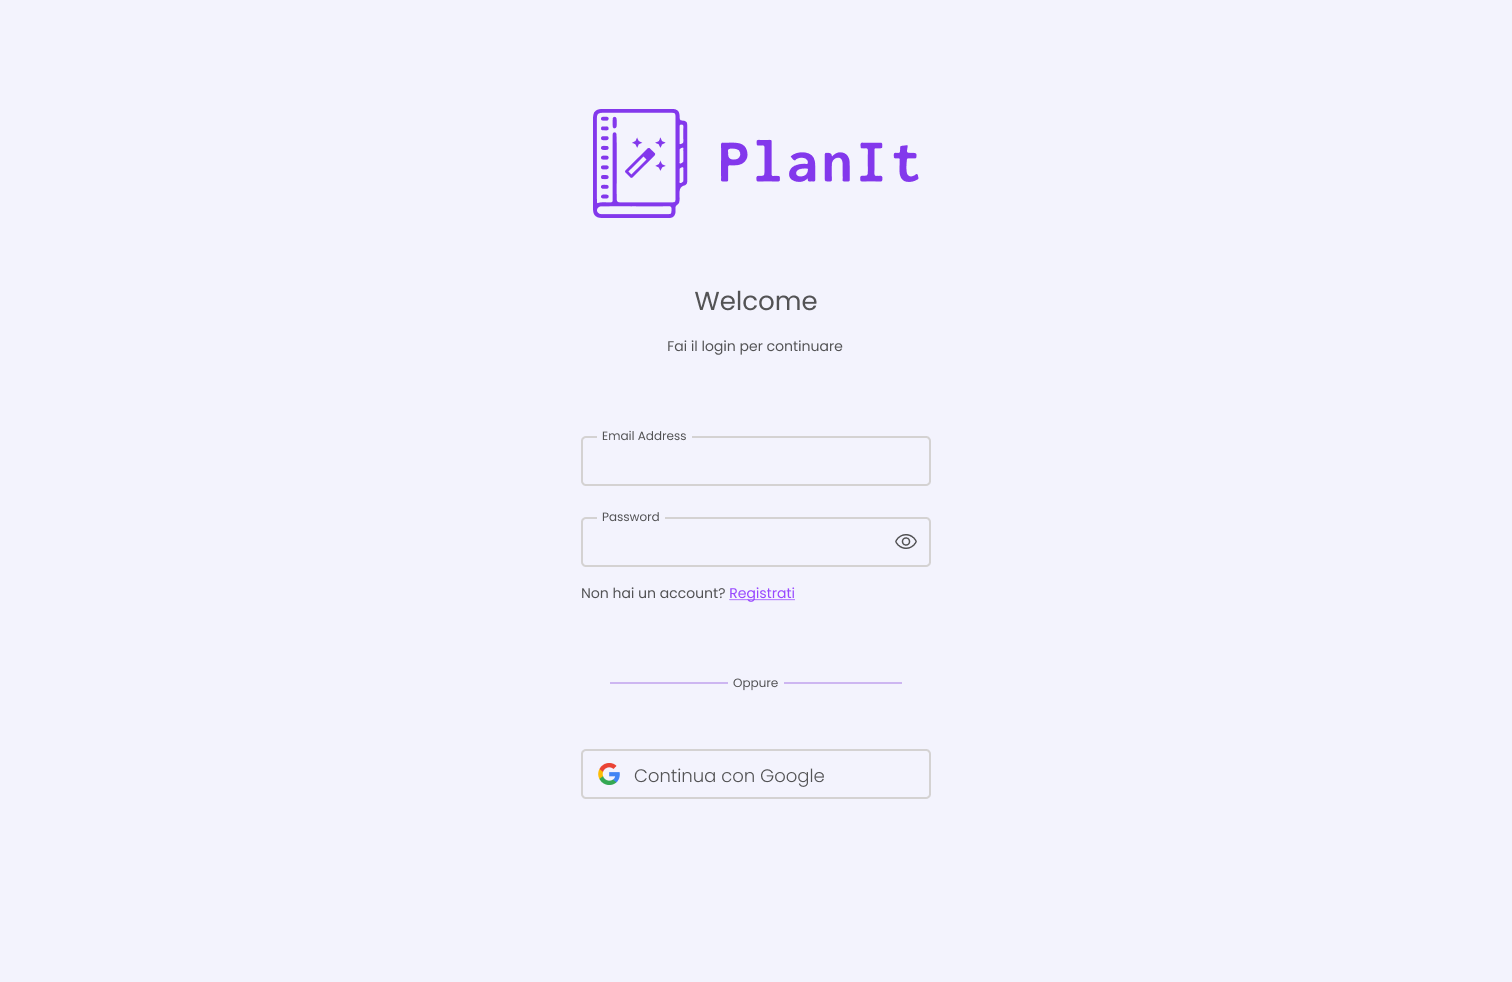
\includegraphics[width=1\textwidth]{img/FrontEnd/Login.png}}
        \caption{Figura 1: schermata quando si apre il sito PlanIt}
    \end{figure}
    \begin{listaPersonale2}{FE}
        \elemento[SCHERMATA RESET PASSWORD]{fe:1.1}
        \begin{figure}[H]
            \centering
            \href{https://www.figma.com/proto/cO66hx25OizBABGtWp8XlT/Planify?node-id=266%3A875&scaling=scale-down&page-id=0%3A1&starting-point-node-id=25%3A82}{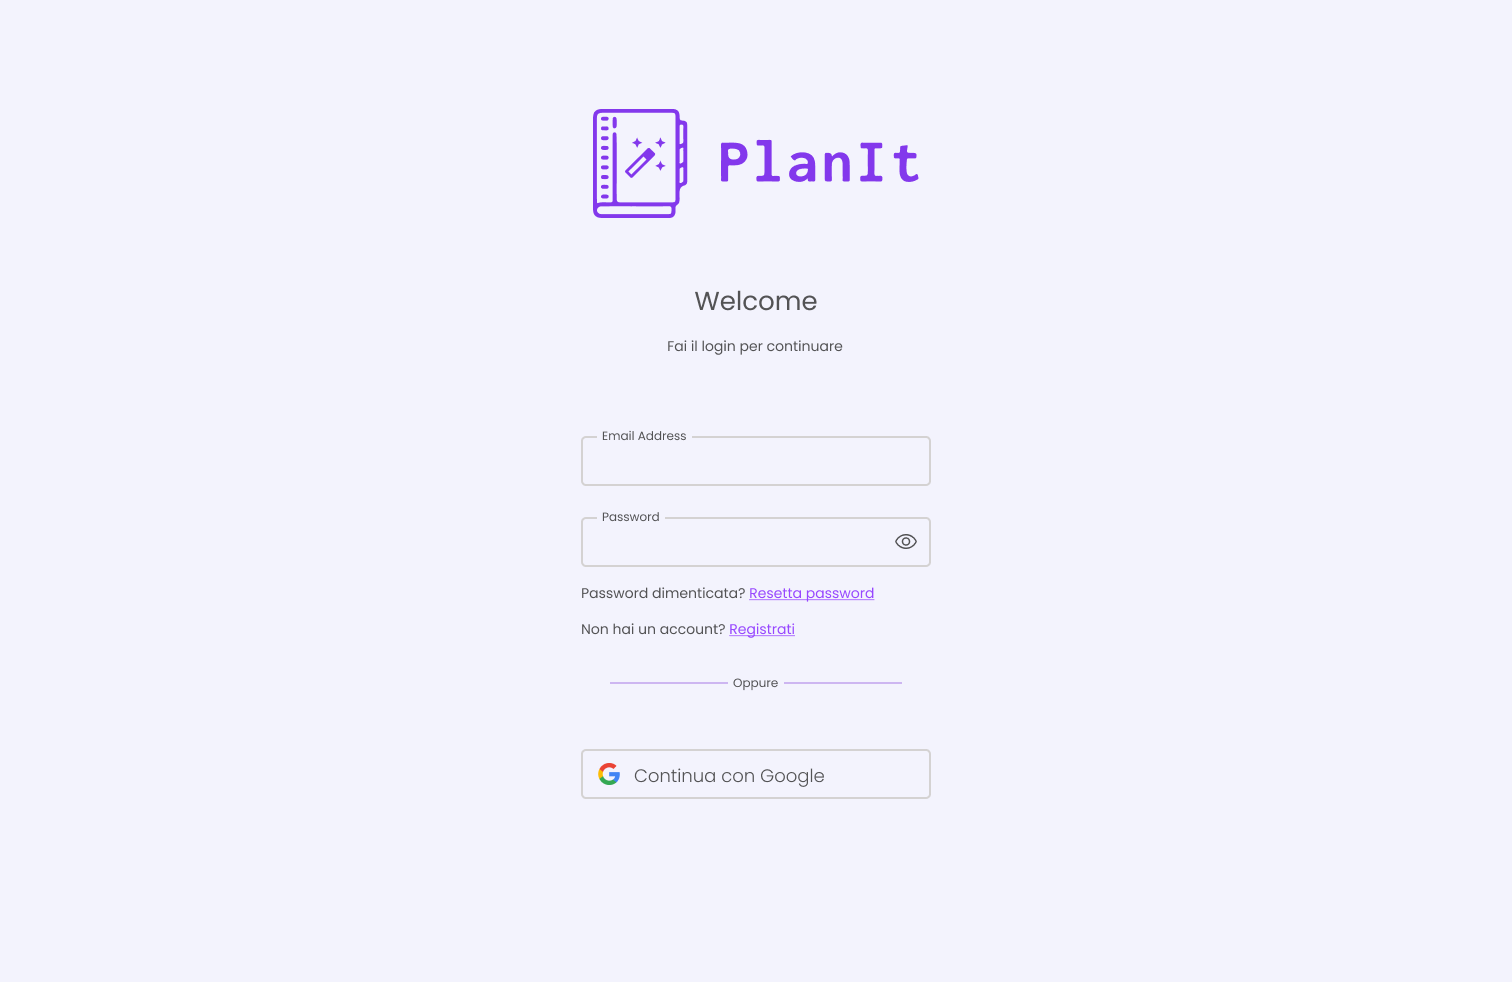
\includegraphics[width=1\textwidth]{img/FrontEnd/ResettaPssw.png}}
            \caption{Figura 1.1: schermata che appare quando si sbaglia più volte una password}
        \end{figure}

        \begin{comment}\begin{figure}%[5]
            \href{https://www.figma.com/proto/cO66hx25OizBABGtWp8XlT/Planify?node-id=266%3A875&scaling=scale-down&page-id=0%3A1&starting-point-node-id=25%3A82}{%
                \parbox{\textwidth}{
                    \centering
                    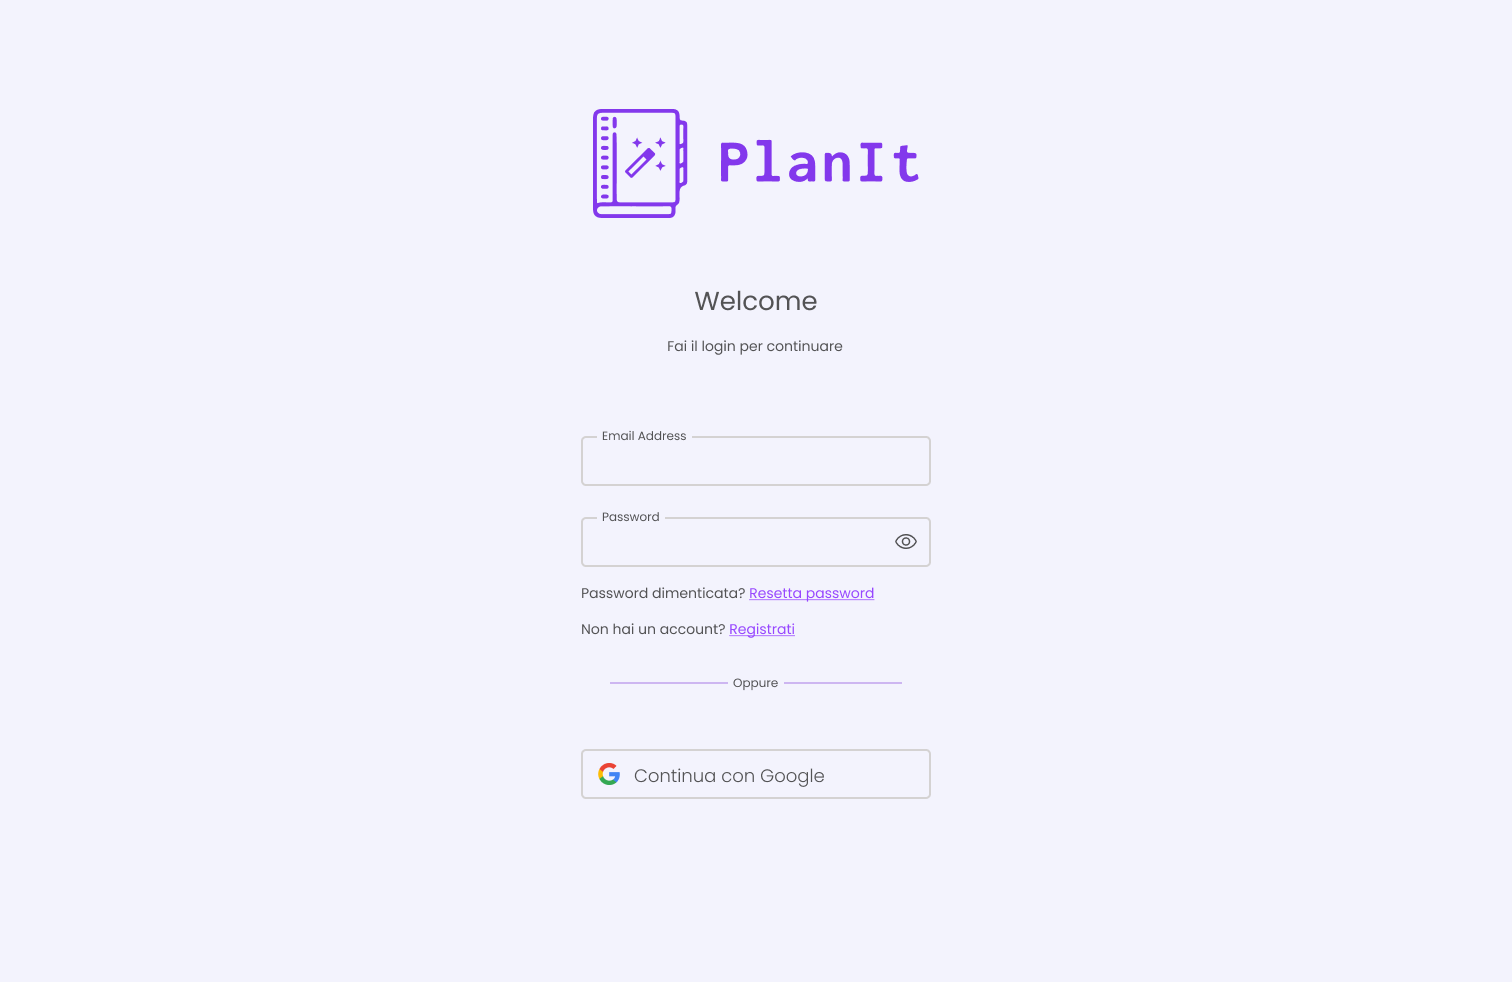
\includegraphics[width=1\textwidth]{img/FrontEnd/ResettaPssw.png}
                    \caption{Figura 1.1: schermata che appare quando si sbaglia più volte una password}
                }
            }
        \end{figure}
        \end{comment}

    \end{listaPersonale2}

    \pagebreak%quasi quasi metterei un pagebreak per ciascuna schermata così per renderlo più ordinato
    
    \elemento [SCHERMATA PRINCIPALE] {fe:2} Questa \href{https://www.figma.com/proto/cO66hx25OizBABGtWp8XlT/Planify?node-id=25%3A82&scaling=scale-down&page-id=0%3A1&starting-point-node-id=25%3A82}{schermata} è la schermata principale della piattaforma PlanIt. L’utente, dopo aver fatto l’accesso al sito oppure proseguito con la modalità demo, giungerà a questa pagina, dove potrà guardare gli eventi posti nella settimana. L’utente ha la possibilità, dal menù al di sopra del calendario, di spostarsi di data sia in mesi che in settimane, visualizzare il calendario per settimana, mese ed anno e accedere agli altri calendari personali e a quelli condivisi (\ref{rf:4.1}). Infine è presente anche il bottone "+” con cui si accede al pop-up di compilazione/aggiunta evento(\ref{rf:5}).
    \begin{figure}[H]
        \centering
        \href{https://www.figma.com/proto/cO66hx25OizBABGtWp8XlT/Planify?node-id=25%3A82&scaling=scale-down&page-id=0%3A1&starting-point-node-id=25%3A82}{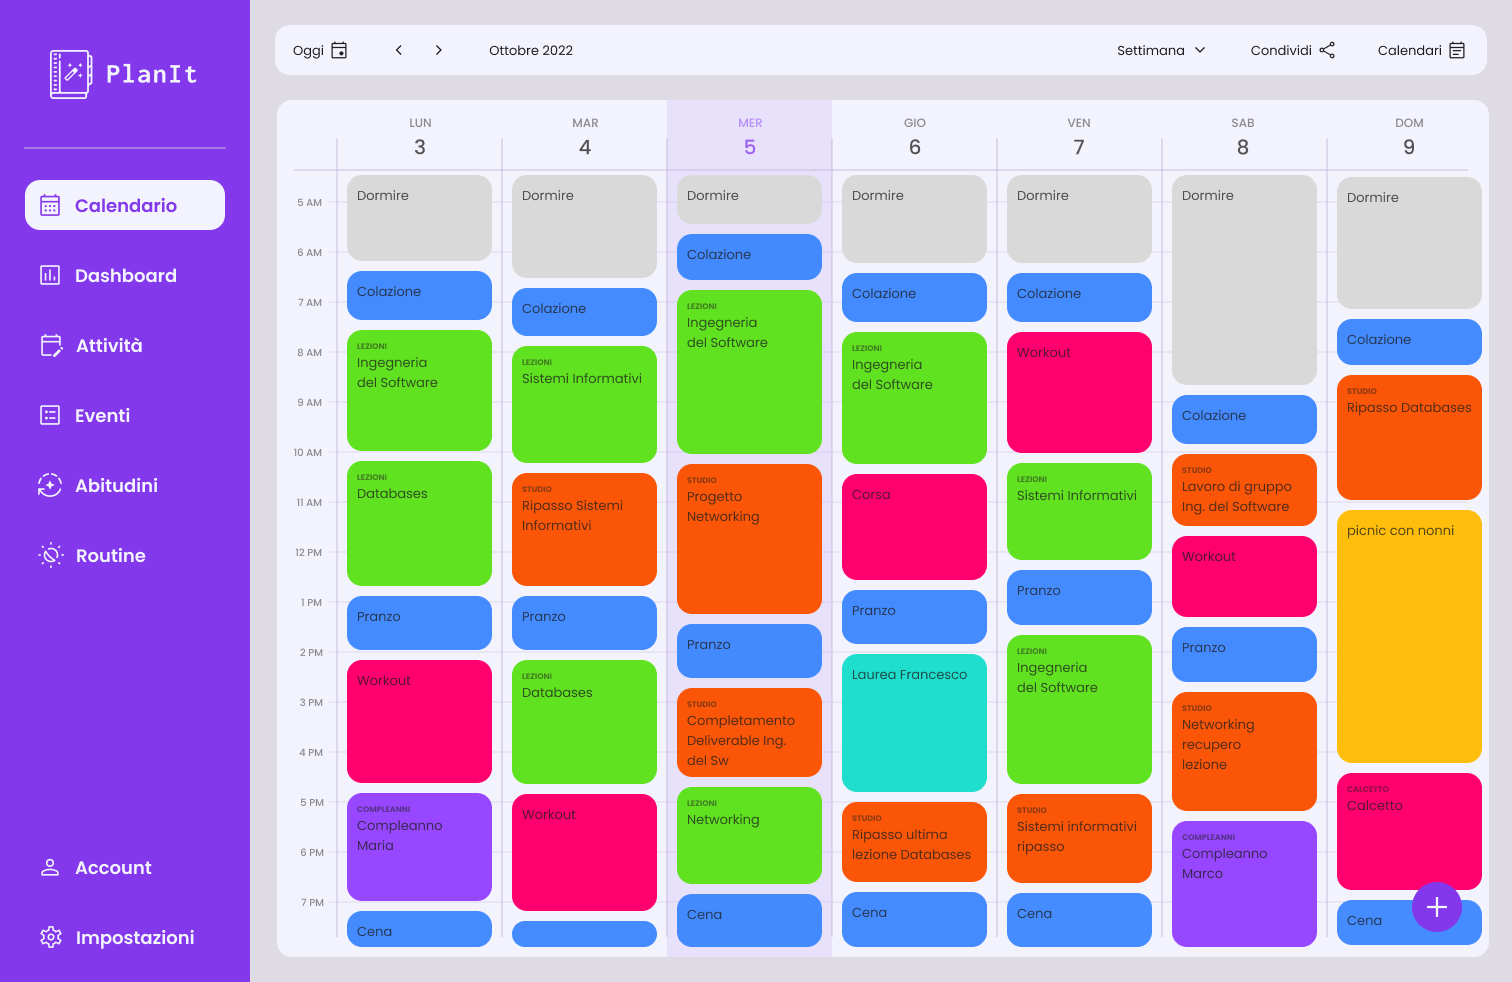
\includegraphics[width=1\textwidth]{img/FrontEnd/Calendar/Calendar.png}}
    \end{figure}
    
    \begin{listaPersonale2}{FE}
        \elemento[SCHERMATA PRINCIPALE-CALENDARI]{fe:2.1} Grazie alla sezione \href{https://www.figma.com/proto/cO66hx25OizBABGtWp8XlT/Planify?node-id=25%3A82&scaling=scale-down&page-id=0%3A1&starting-point-node-id=25%3A82}{"Calendari"}  l’utente aprirà una sezione da dove può gestire i propri calendari e i calendari condivisi di altre persone (\ref{rf:4.1}). I calendari condivisi da altri utenti sono indicati con una piccola immagine stereotipata di persone, alla destra del loro nome.
    \end{listaPersonale2}
    \begin{figure}[H]
        \centering
        \href{https://www.figma.com/proto/cO66hx25OizBABGtWp8XlT/Planify?node-id=25%3A82&scaling=scale-down&page-id=0%3A1&starting-point-node-id=25%3A82}{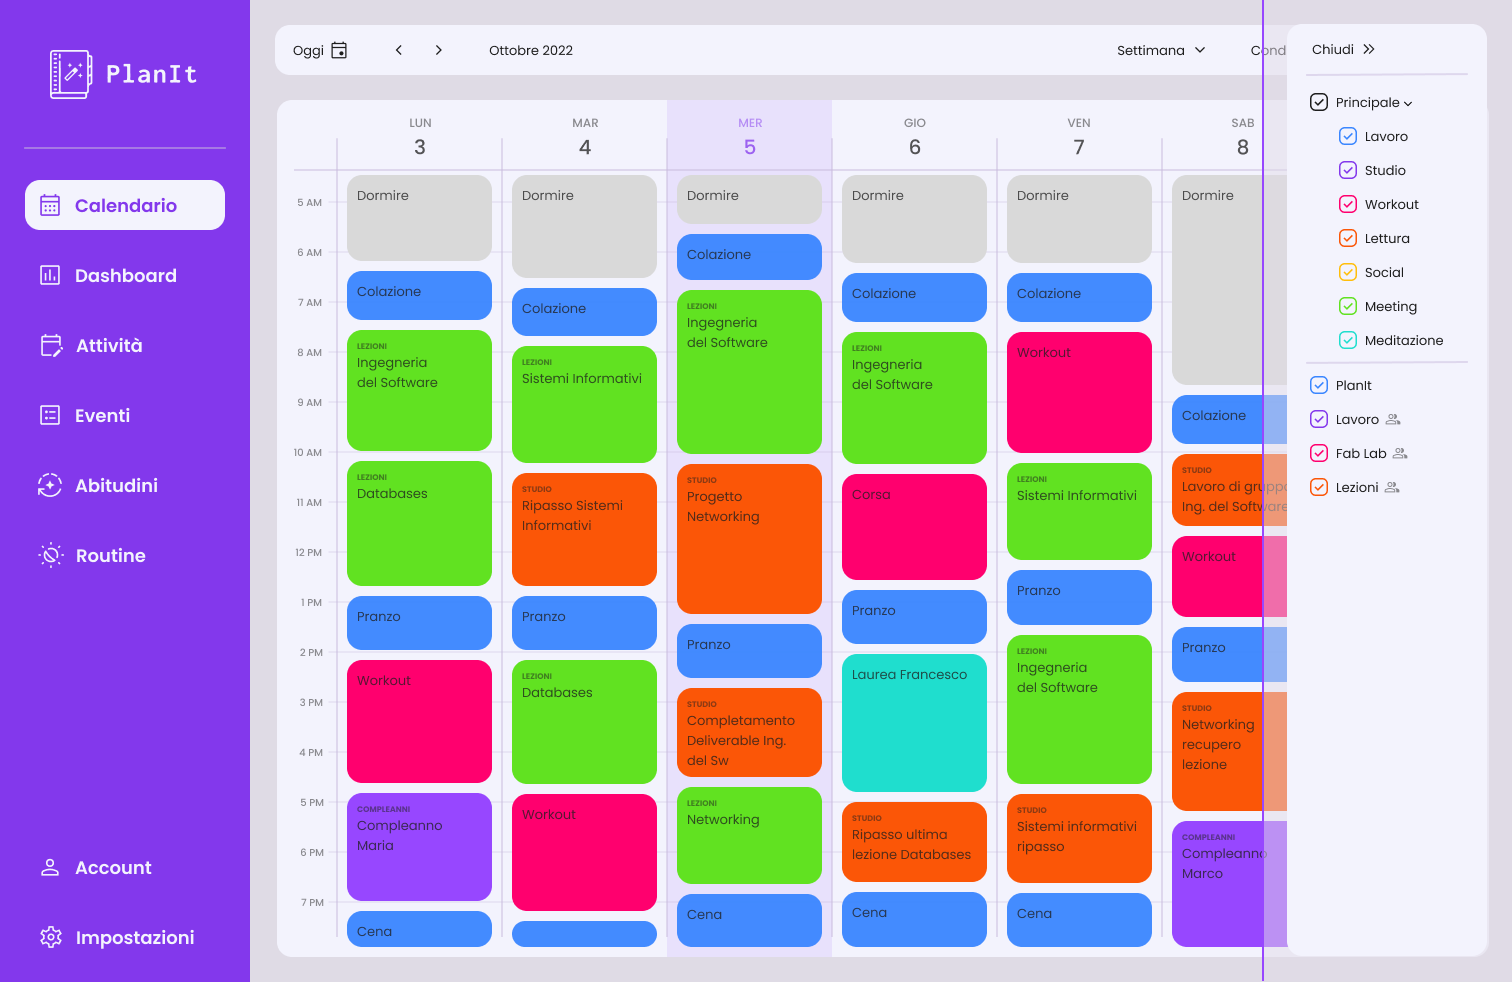
\includegraphics[width=0.9\textwidth,height=0.33\textheight]{img/FrontEnd/Calendar/CalendarCondivisi.png}}
    \end{figure}

    \pagebreak
    \elemento[DASHBOARD] {fe:3} L’utente, nella \href{https://www.figma.com/proto/cO66hx25OizBABGtWp8XlT/Planify?node-id=84%3A178&scaling=scale-down&page-id=0%3A1&starting-point-node-id=25%3A82}{dashboard}, può osservare le informazioni principali riguardo al proprio calendario, le sezioni presenti sono: "Attività svolte questa settimana", "Situazione scadenza attività" e "Attività svolte oggi" con "Grafico attività svolte".
    \begin{figure}[H]
        \centering
        \href{https://www.figma.com/proto/cO66hx25OizBABGtWp8XlT/Planify?node-id=84%3A178&scaling=scale-down&page-id=0%3A1&starting-point-node-id=25%3A82}{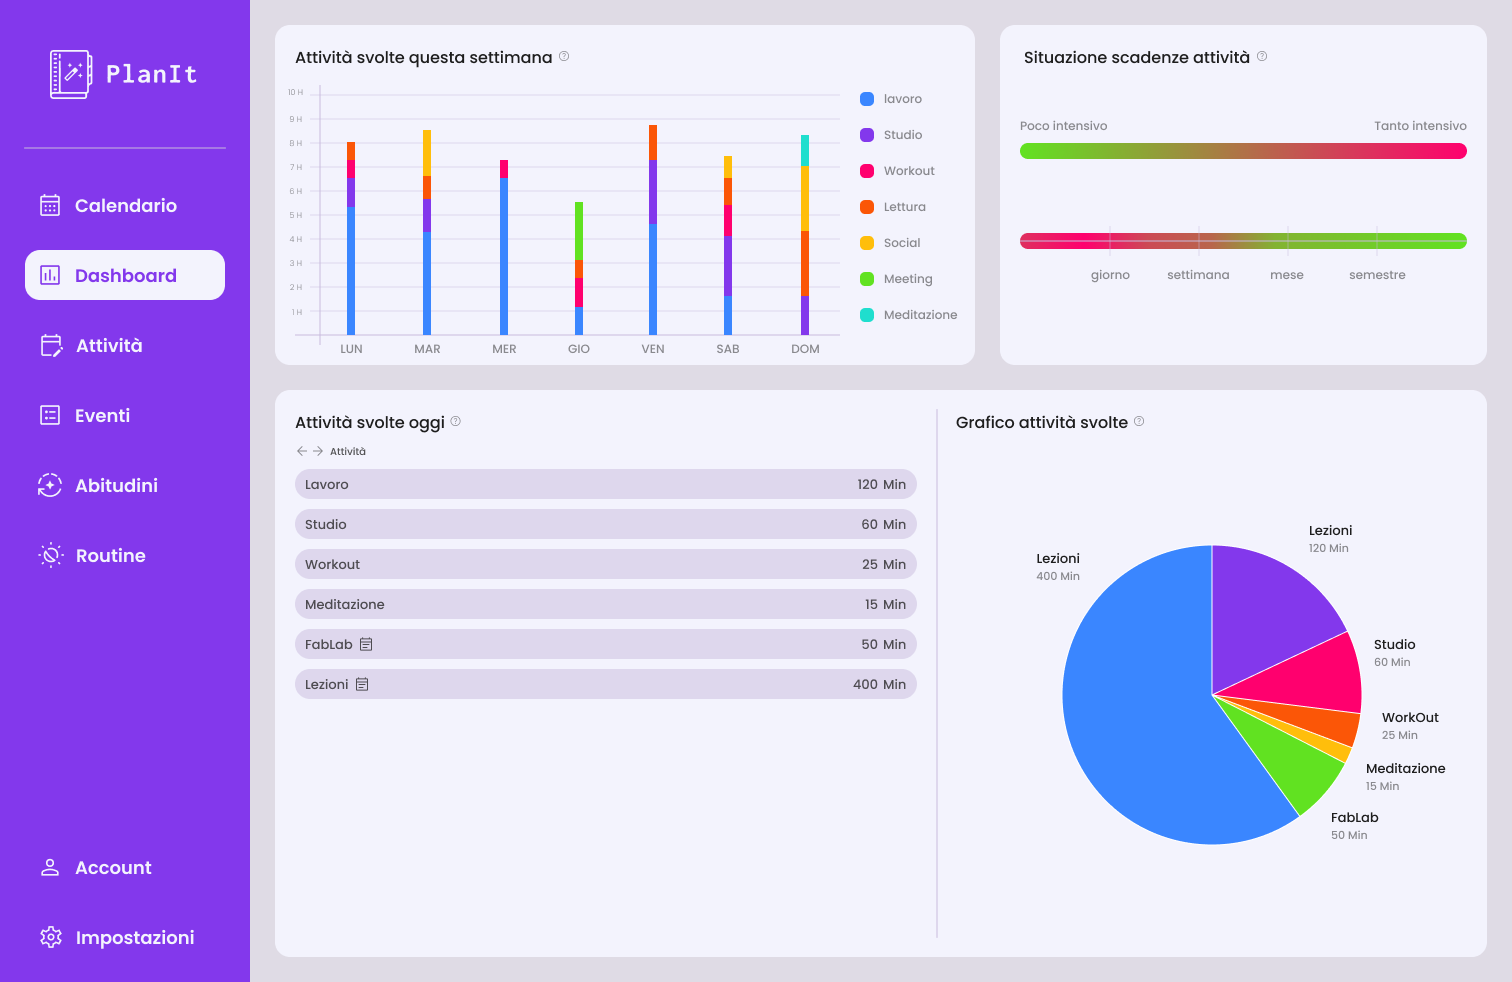
\includegraphics[width=1\textwidth]{img/FrontEnd/Dashboard/Dashboard.png}}
    \end{figure}

    
    \begin{listaPersonale2}{FE}
        \elemento[ATTIVITA' SVOLTE QUESTA SETTIMANA] {fe:3.1} Nella sezione “Attività svolte questa settimana” viene mostrato un grafico a barre delle varie attività svolte per ogni giorno della settimana (\ref{rf:9}); l’altezza delle barre corrisponde al quantitativo di ore dedicate a quell’attività.
        \begin{figure}[H]
            \centering
            \href{https://www.figma.com/proto/cO66hx25OizBABGtWp8XlT/Planify?node-id=84%3A178&scaling=scale-down&page-id=0%3A1&starting-point-node-id=25%3A82}{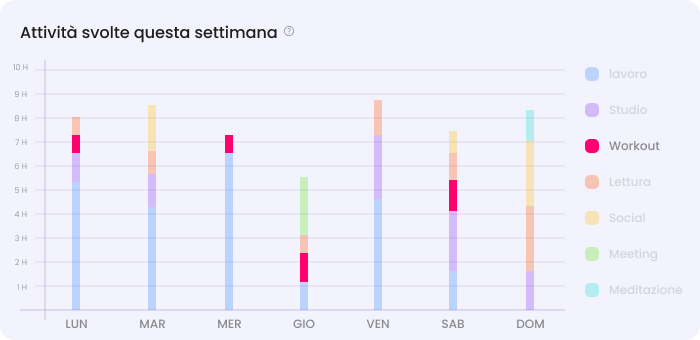
\includegraphics[width=0.6\textwidth,height=0.18\textheight]{img/FrontEnd/Dashboard/graficoBarre.png}}
            \caption{Figura 3.1: come appare il grafico quando si preme una delle attività della mia legenda}
        \end{figure}
        \pagebreak
        \elemento[SITUAZIONE SCADENZA ATTIVITA'] {fe:3.2}
        Nella sezione “Situazione scadenze attività” è presente in basso una heatmap riguardo al tempo che deve essere dedicato ogni giorno per rispettare le varie deadline (\ref{rf:9}). La legenda sopra la heatmap mostra che più si è tendenti al colore rosso, più ore si devono  impiegare nello specifico periodo di tempo.
        \begin{figure}[H]
            \centering
            \href{https://www.figma.com/proto/cO66hx25OizBABGtWp8XlT/Planify?node-id=84%3A178&scaling=scale-down&page-id=0%3A1&starting-point-node-id=25%3A82}{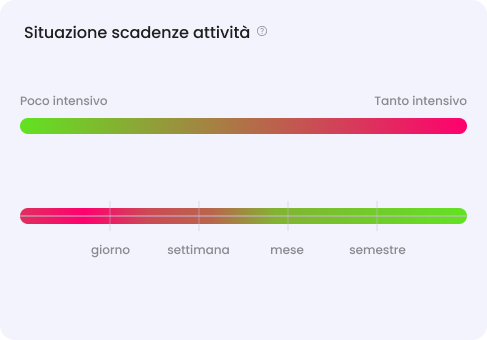
\includegraphics[width=0.45\textwidth,height=0.18\textheight]{img/FrontEnd/Dashboard/heatMap.png}}
        \end{figure}
        
        \elemento [ATTIVITA’ SVOLTE OGGI e GRAFICO ATTIVITA' SVOLTE] {fe:3.3} Nella sezione “Attività svolte oggi” è presente una lista delle attività della giornata, da cui si possono ottenere anche le varie sottoattività. 
        La sezione “Attività svolte oggi” è sincronizzata con il grafico a torta presente nel “Grafico attività svolte” (\ref{rf:9}). Il grafico presenta le attività selezionate in “Attività svolte oggi” con una dimensione proporzionata al tempo da spendere.

        \begin{figure}[H]
            \centering
            \href{https://www.figma.com/proto/cO66hx25OizBABGtWp8XlT/Planify?node-id=84%3A178&scaling=scale-down&page-id=0%3A1&starting-point-node-id=25%3A82}{\includegraphics[width=0.72\textwidth,height=0.2\textheight]{img/FrontEnd/Dashboard/selezionatoAttività.png}}
            \caption{Figura 3.3.1: schermata che appare quando si mette il puntatore sopra una delle raggruppamenti della lista}
        \end{figure}

        \begin{figure}[H]
            \centering
            \href{https://www.figma.com/proto/cO66hx25OizBABGtWp8XlT/Planify?node-id=84%3A178&scaling=scale-down&page-id=0%3A1&starting-point-node-id=25%3A82}{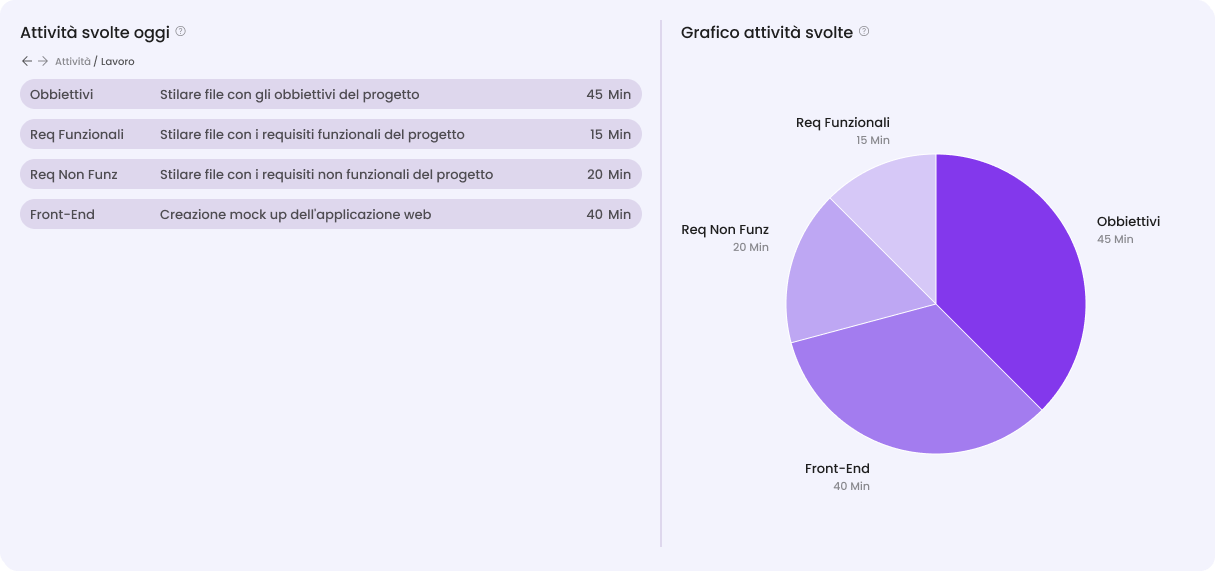
\includegraphics[width=0.72\textwidth,height=0.2\textheight]{img/FrontEnd/Dashboard/Dashboard3.png}}
            \caption{Figura 3.3.2: schermata quando si seleziona una delle attività della lista}
        \end{figure}
           
    \end{listaPersonale2}
    \pagebreak
    \elemento [SCHERMATA ATTIVITA'] {fe:4} Nella \href{https://www.figma.com/proto/cO66hx25OizBABGtWp8XlT/Planify?node-id=159%3A277&scaling=scale-down&page-id=0%3A1&starting-point-node-id=25%3A82}{schermata attività} è presente una tabella delle attività della giornata con le varie informazioni, ovvero: titolo, descrizione, categoria, priorità, durata (\ref{rf:5}), posizione (\ref{rf:8.2}) e difficoltà. Inoltre ci sono dei tasti con cui si può ritardare (\ref{rf:10}), eliminare (\ref{rf:5})l'attività e, infine, un tasto per indicare di averla completata. A fine giornata di default tutti gli impegni sono posti come completati; per modificare tale opzione deve intervenire l’utente.
    \begin{figure}[H]
        \centering
        \href{https://www.figma.com/proto/cO66hx25OizBABGtWp8XlT/Planify?node-id=159%3A277&scaling=scale-down&page-id=0%3A1&starting-point-node-id=25%3A82}{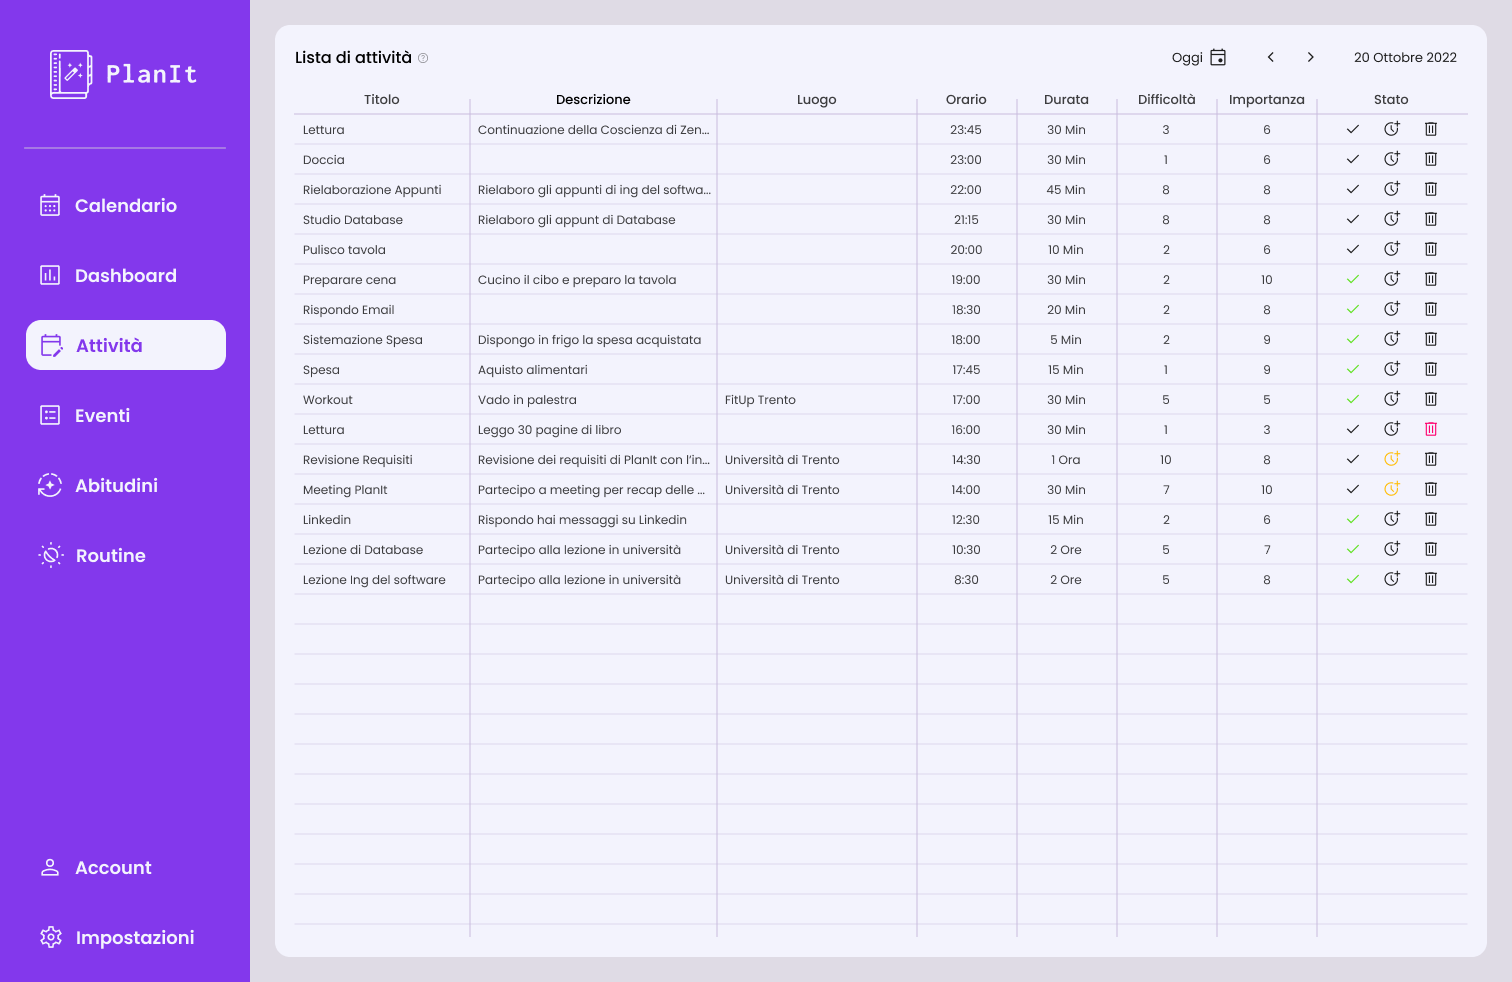
\includegraphics[width=1\textwidth]{img/FrontEnd/Attivita/Attivita.png}}
        \caption {Figura 4: le spunte verdi indicano il completamento dell'evento; l'orologio giallo indica il ritardo nel compiere l'evento; il cestino l'eliminazione dell'evento}
    \end{figure}
    \pagebreak
    \elemento [SCHERMATA EVENTI] {fe:5} Nella \href{https://www.figma.com/proto/cO66hx25OizBABGtWp8XlT/Planify?node-id=160%3A290&scaling=scale-down&page-id=0%3A1&starting-point-node-id=25%3A82}{schermata eventi} sono presenti tutti i comandi che riguardano la compilazione ed eliminazione di eventi (\ref{rf:5}), calendari (\ref{rf:4.2}) e raggruppamenti (RF\ref{rf:5.9}).
    Nella sezione sottostante, è presente una lista dei vari calendari, eventi e raggruppamenti, che selezionati una alla volta aprono i rispettivi form di modifica, dove sono presenti tutti i campi citati in (\ref{rf:5}) per l’aggiunta e modifica di impegni e raggruppamenti e (\ref{rf:13}) per la modifica e aggiunta di calendari. Mediante un'azione di "drag and drop" è possibile spostare l'elemento selezionato da una posizione all'altra della lista.
    %qua dipende dalla formattazione andrebbe un clearpage
    \begin{figure}[H]
        \centering
        \href{https://www.figma.com/proto/cO66hx25OizBABGtWp8XlT/Planify?node-id=160%3A290&scaling=scale-down&page-id=0%3A1&starting-point-node-id=25%3A82}{\includegraphics[width=1\textwidth]{img/FrontEnd/Eventi/SottoAttività.png}}
        \caption{Figura 5: schermata quando si apre la sezione "Eventi"}
    \end{figure}
    \begin{figure}[H]
        \centering
        \href{https://www.figma.com/proto/cO66hx25OizBABGtWp8XlT/Planify?node-id=160%3A290&scaling=scale-down&page-id=0%3A1&starting-point-node-id=25%3A82}{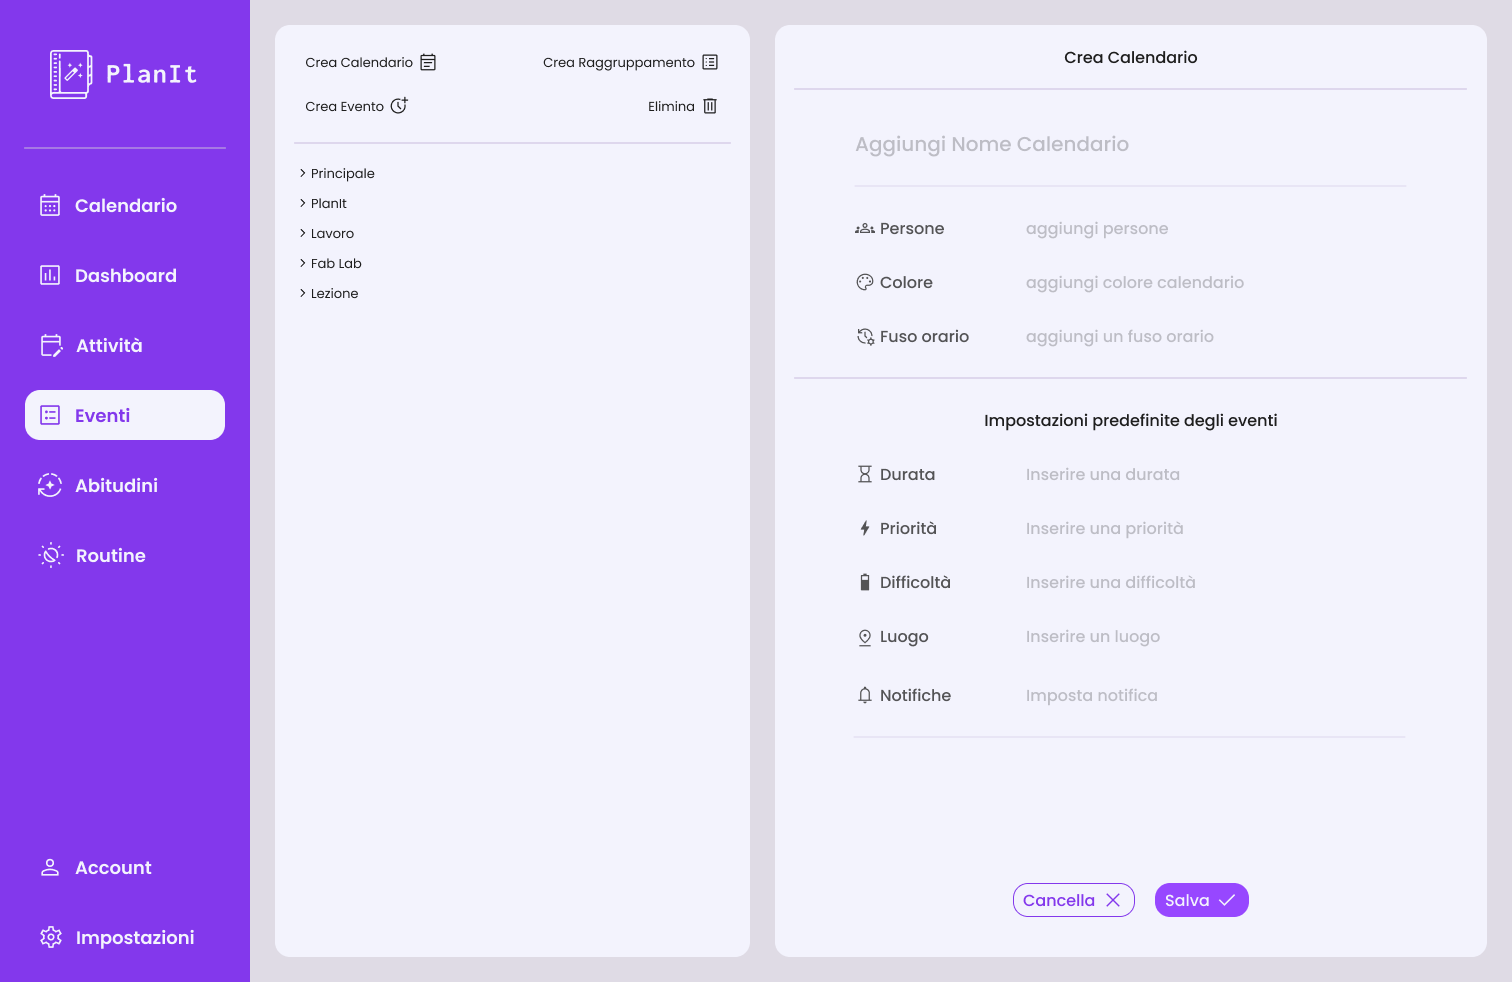
\includegraphics[width=1\textwidth]{img/FrontEnd/Eventi/Calendario/CreaCalendario.png}}
        \caption{Figura 5: schermata quando si seleziona uno dei comandi o un'attività della lista}
    \end{figure}
    \begin{listaPersonale2}{FE}
        
        \elemento[SCHERMATA CREA/MODIFICA EVENTO] {fe:5.1}

        \begin{center} 
            \begin{figure}[H]
            \centering        
            \href{https://www.figma.com/proto/cO66hx25OizBABGtWp8XlT/Planify?node-id=160%3A290&scaling=scale-down&page-id=0%3A1&starting-point-node-id=25%3A82}{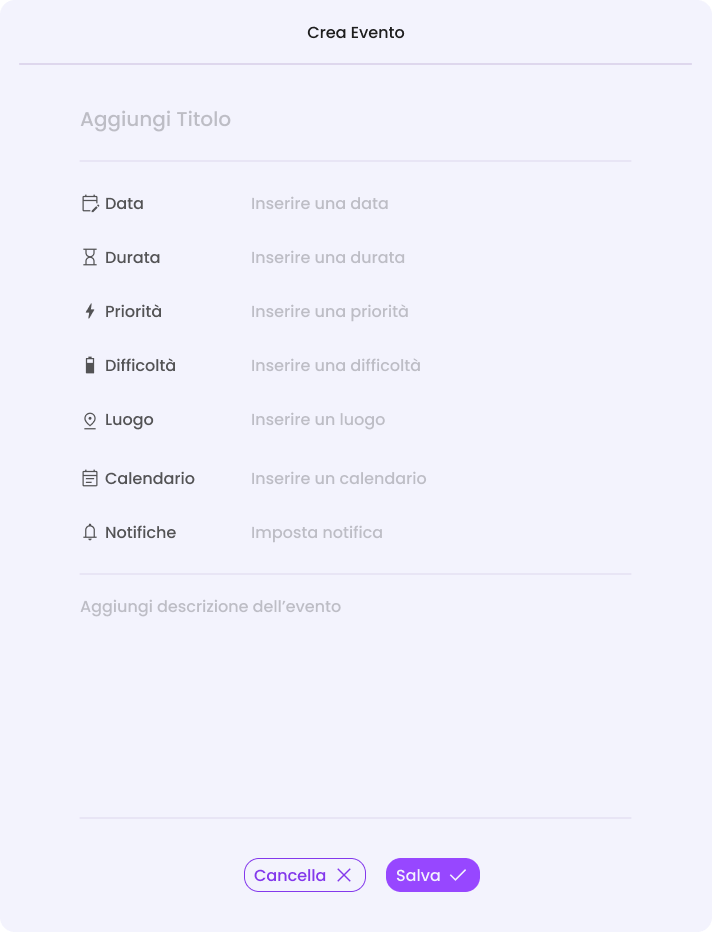
\includegraphics[width=0.49\textwidth,height=0.35\textheight]{img/FrontEnd/Eventi/Evento/CreaEvento.png}}
            \centering
            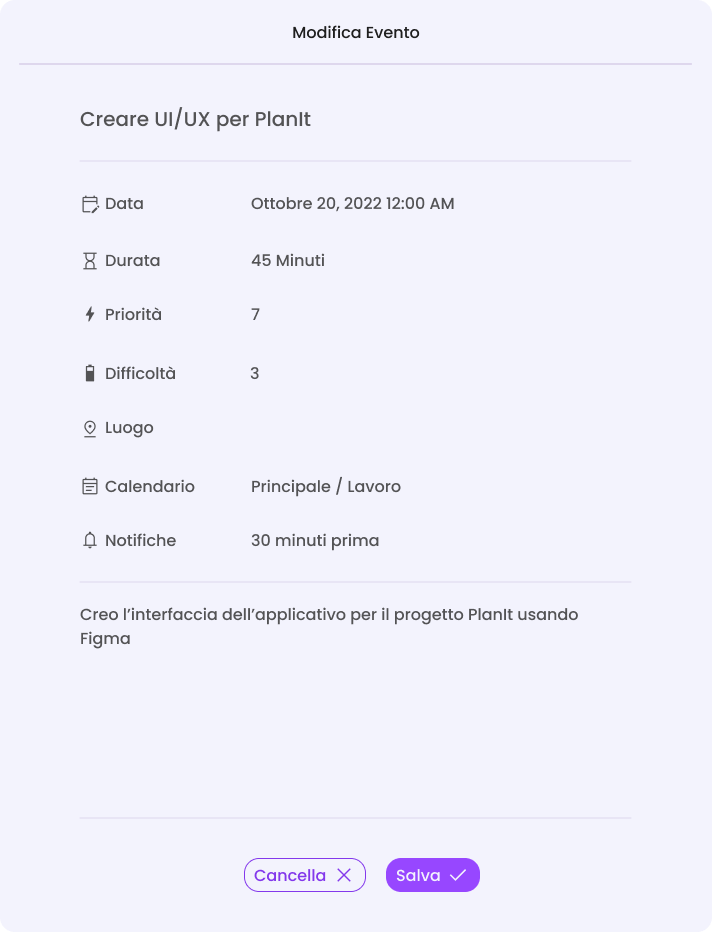
\includegraphics[width=0.49\textwidth,height=0.35\textheight]{img/FrontEnd/Eventi/Evento/ModificaEvento.png}
            \end{figure}
        \end{center}

        
        \elemento[SCHERMATA CREA/MODIFICA RAGGRUPPAMENTO] {fe:5.2}

        \begin{center} 
            \begin{figure}[H]
            \centering
            \href{https://www.figma.com/proto/cO66hx25OizBABGtWp8XlT/Planify?node-id=160%3A290&scaling=scale-down&page-id=0%3A1&starting-point-node-id=25%3A82}{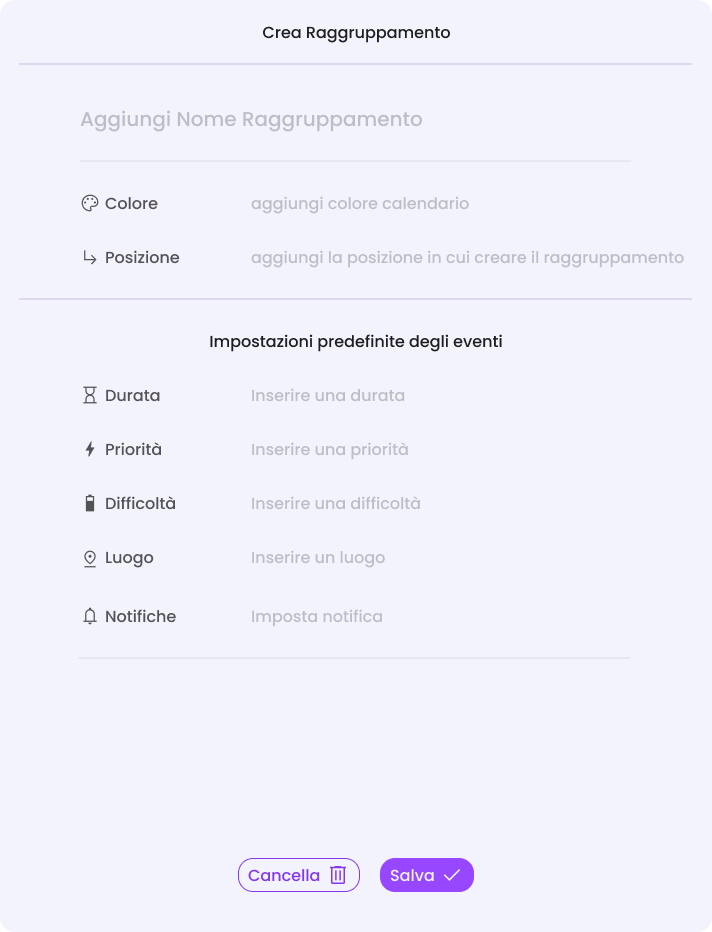
\includegraphics[width=0.49\textwidth,height=0.35\textheight]{img/FrontEnd/Eventi/Raggruppamento/CreaRaggruppamento.png}}
            \centering
            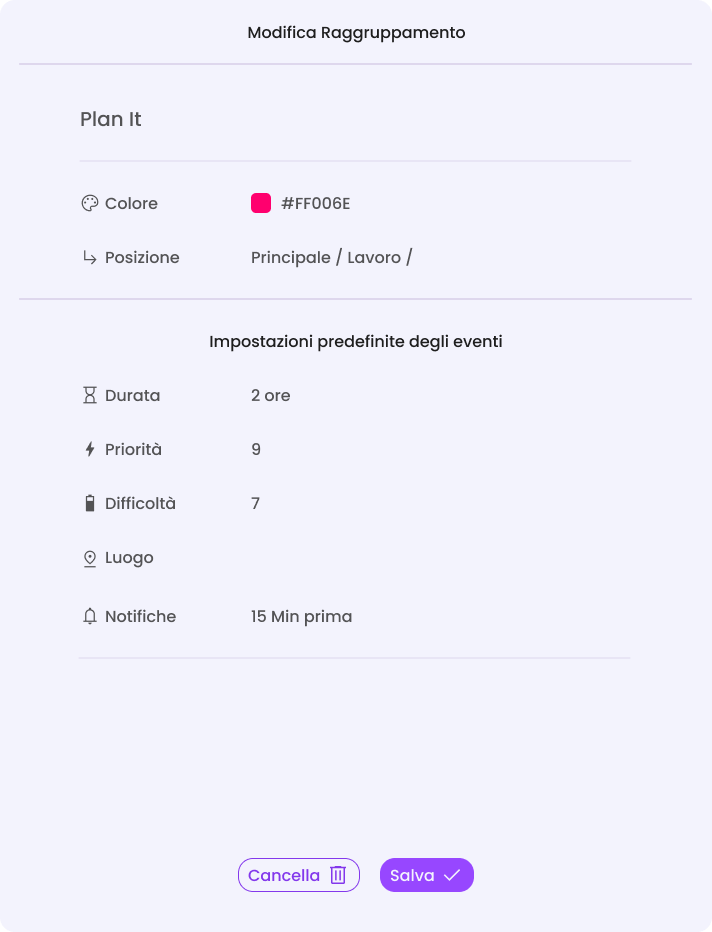
\includegraphics[width=0.49\textwidth,height=0.35\textheight]{img/FrontEnd/Eventi/Raggruppamento/ModificaRaggruppamento.png}
            \end{figure}
        \end{center}
        \pagebreak
        \elemento[SCHERMATA CREA/MODIFICA CALENDARIO] {fe:5.3}

        \begin{center} 
            \begin{figure}[H]
            \centering
            \href{https://www.figma.com/proto/cO66hx25OizBABGtWp8XlT/Planify?node-id=160%3A290&scaling=scale-down&page-id=0%3A1&starting-point-node-id=25%3A82}{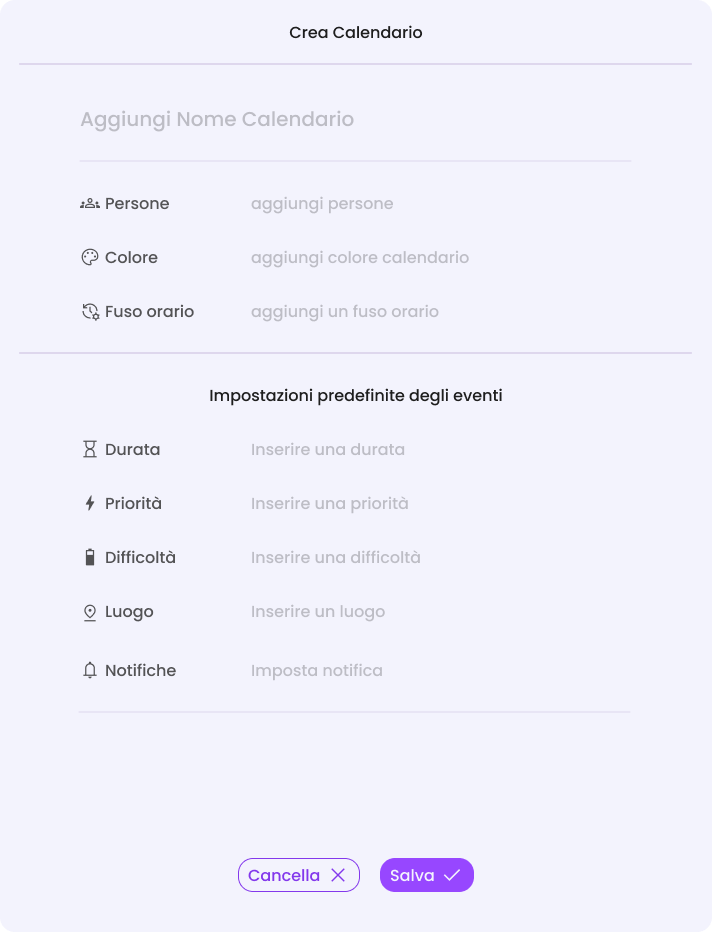
\includegraphics[width=0.49\textwidth,height=0.35\textheight]{img/FrontEnd/Eventi/Calendario/CreaCalendario1.png}}
            \centering
            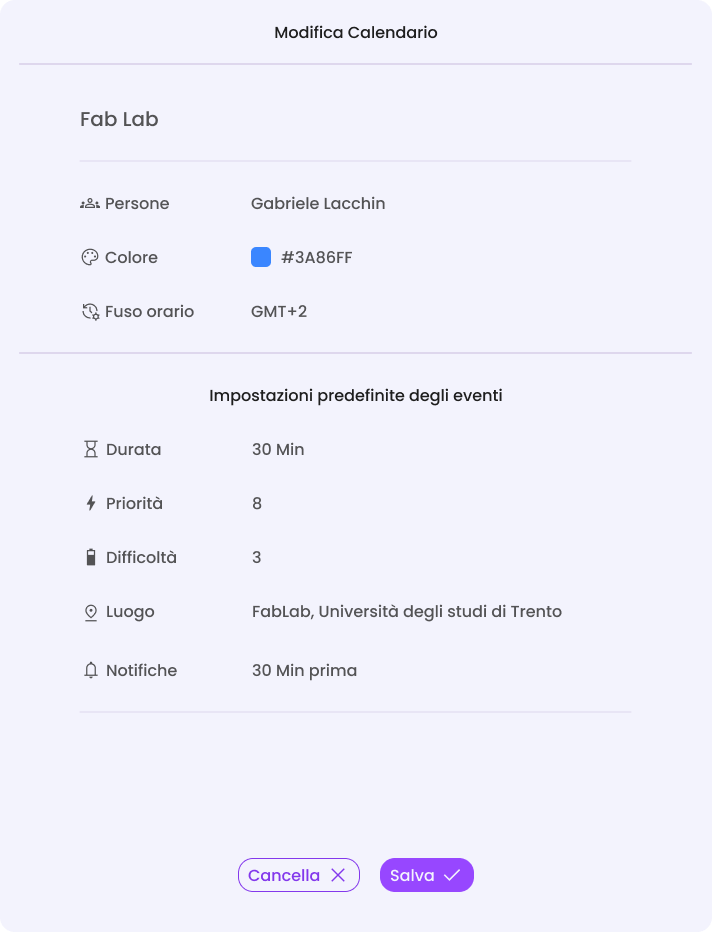
\includegraphics[width=0.49\textwidth,height=0.35\textheight]{img/FrontEnd/Eventi/Calendario/ModificaCalendario.png}
            \end{figure}
        \end{center}
        
    \end{listaPersonale2}
    \pagebreak
    \elemento [SCHERMATA ABITUDINI] {fe:6} Nella schermata          \href{https://www.figma.com/proto/cO66hx25OizBABGtWp8XlT/Planify?node-id=160%3A399&scaling=scale-down&page-id=0%3A1&starting-point-node-id=25%3A82}{"Abitudini"} l’utente può visualizzare la lista delle abitudini del proprio calendario. Inoltre, nella sezione di destra, si può aprire un form per la modifica, aggiunta ed eliminazione (\ref{rf:5}) di un'abitudine(RF\ref{rf:5.4}) selezionando una di quest'ultime.
    \begin{figure}[H]
        \centering
        \href{https://www.figma.com/proto/cO66hx25OizBABGtWp8XlT/Planify?node-id=160%3A399&scaling=scale-down&page-id=0%3A1&starting-point-node-id=25%3A82}{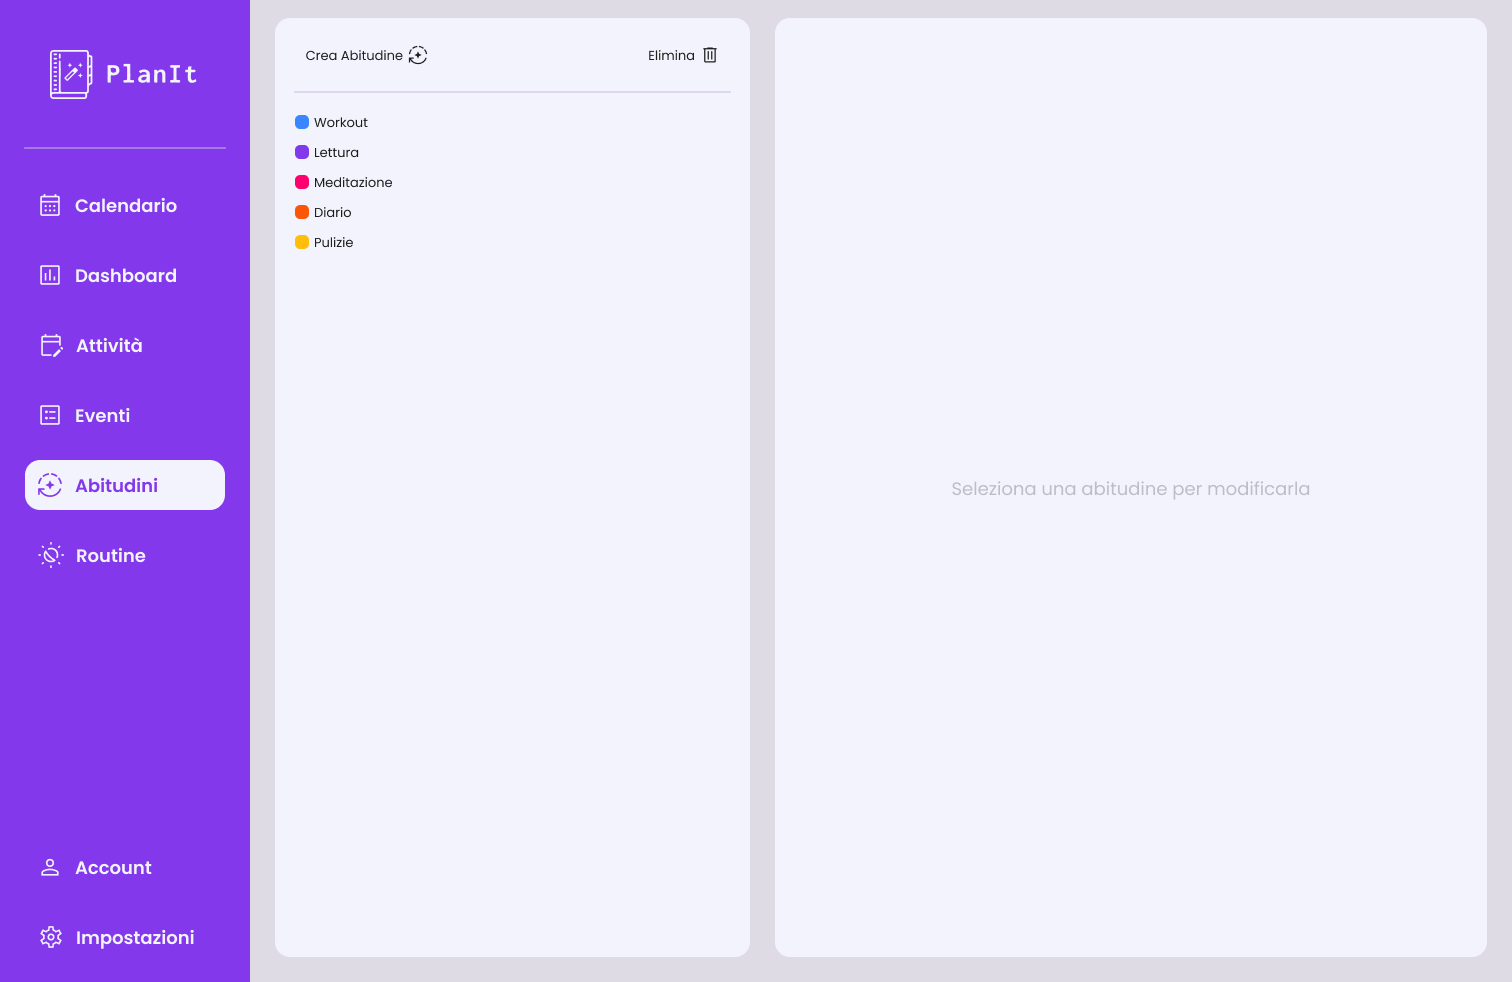
\includegraphics[width=1\textwidth]{img/FrontEnd/Abitudini/Abitudini.png}}
        \caption{Figura 6: schermata quando si apre la sezione "Abitudini"}
    \end{figure}

    \begin{figure}[H]
        \centering
        \href{https://www.figma.com/proto/cO66hx25OizBABGtWp8XlT/Planify?node-id=160%3A399&scaling=scale-down&page-id=0%3A1&starting-point-node-id=25%3A82}{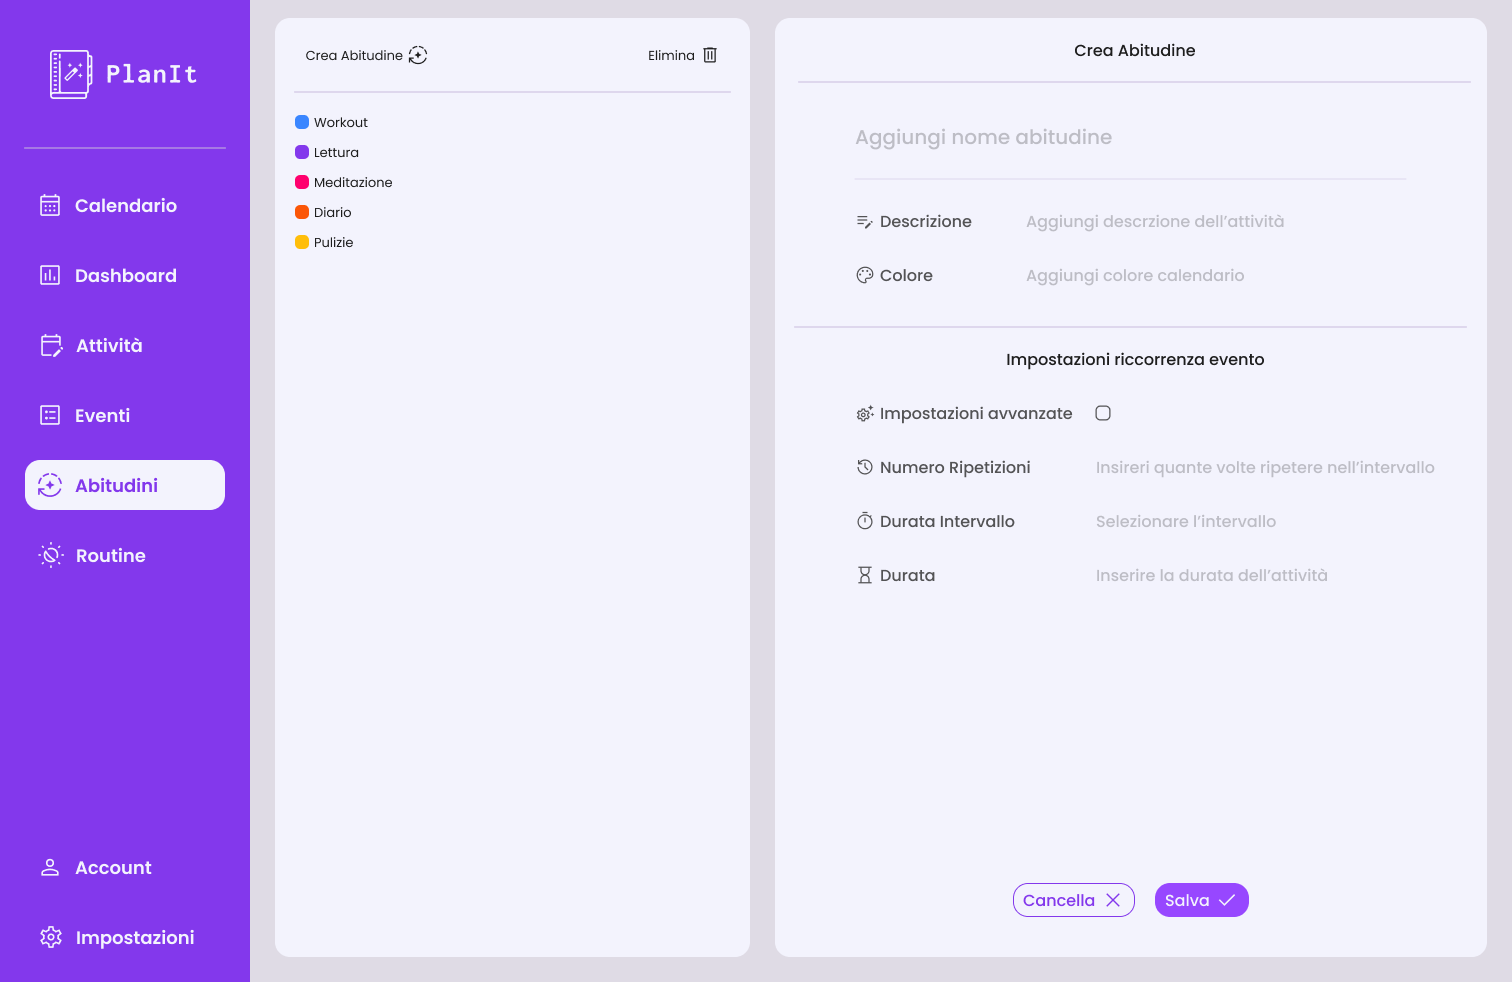
\includegraphics[width=1\textwidth]{img/FrontEnd/Abitudini/CreaAbitudiniMain.png}}
        \caption{Figura 6: schermata quando si seleziona uno dei comandi o un'abitudine della lista}
    \end{figure}

    \begin{listaPersonale2}{FE}
        
        \elemento[SCHERMATA CREA ABITUDINI E IMPOSTAZIONI AVANZATE]{fe:6.1}
        \begin{center} 
            \begin{figure}[H]
            \centering
            \href{https://www.figma.com/proto/cO66hx25OizBABGtWp8XlT/Planify?node-id=160%3A399&scaling=scale-down&page-id=0%3A1&starting-point-node-id=25%3A82}{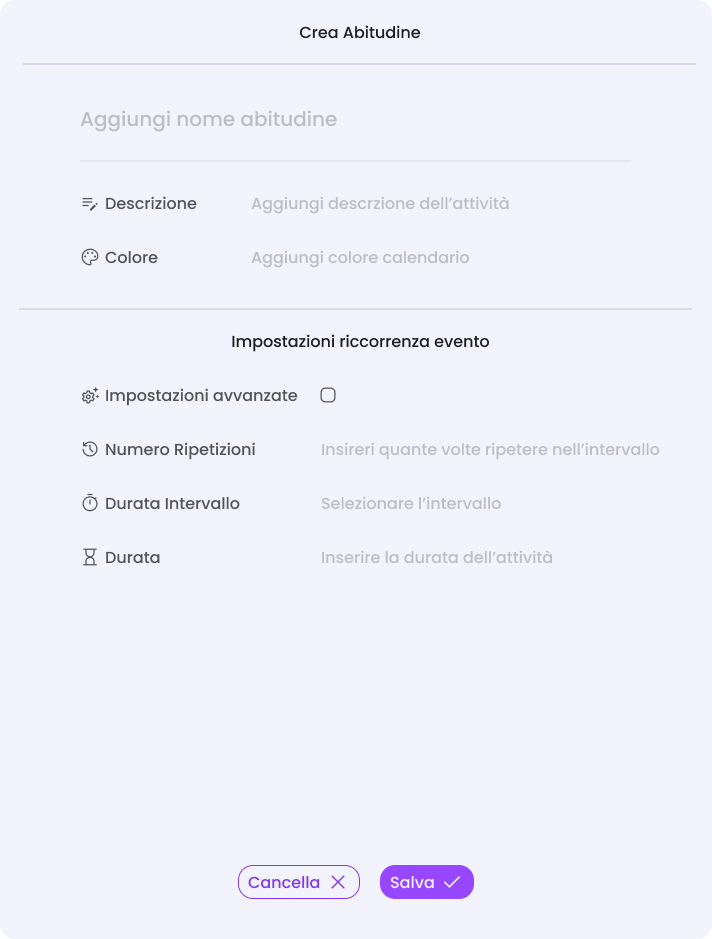
\includegraphics[width=0.49\textwidth,height=0.35\textheight]{img/FrontEnd/Abitudini/Crea/CreaAbitudine.png}}
            \centering
            \href{https://www.figma.com/proto/cO66hx25OizBABGtWp8XlT/Planify?node-id=160%3A399&scaling=scale-down&page-id=0%3A1&starting-point-node-id=25%3A82}{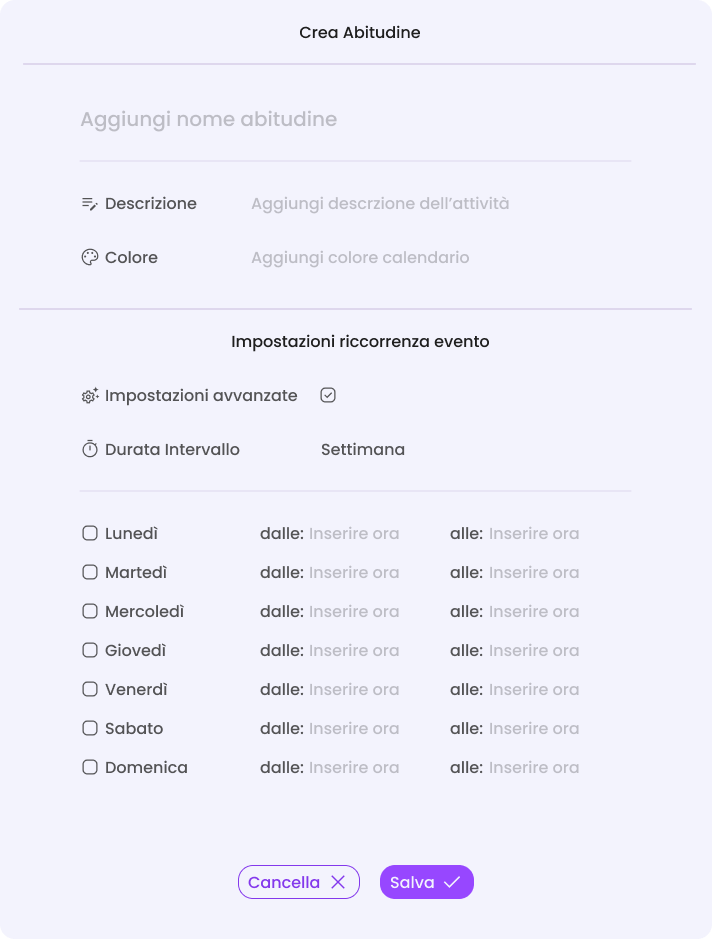
\includegraphics[width=0.49\textwidth,height=0.35\textheight]{img/FrontEnd/Abitudini/Crea/CreaAbitudineAvv.png}}
            \end{figure}
        \end{center}

        \elemento [SCHERMATA MODIFICA ABITUDINI E IMPOSTAZIONI AVANZATE] {fe:6.2}
        \begin{center} 
            \begin{figure}[H]
            \centering
            \href{https://www.figma.com/proto/cO66hx25OizBABGtWp8XlT/Planify?node-id=160%3A399&scaling=scale-down&page-id=0%3A1&starting-point-node-id=25%3A82}{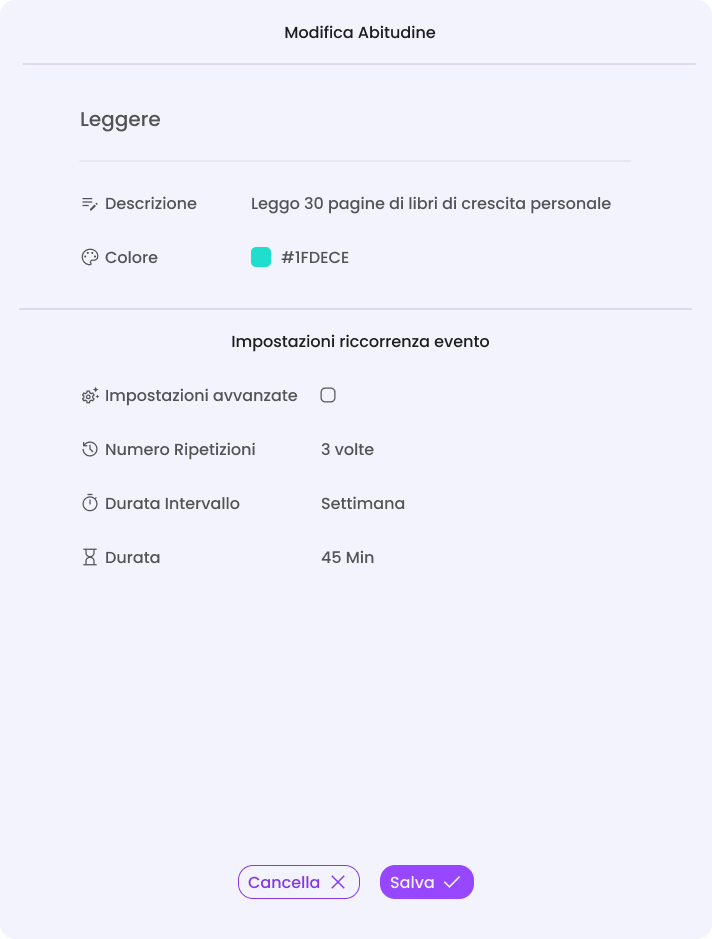
\includegraphics[width=0.49\textwidth,height=0.35\textheight]{img/FrontEnd/Abitudini/Modifica/ModificaAbitudine.png}}
            \centering
            \href{https://www.figma.com/proto/cO66hx25OizBABGtWp8XlT/Planify?node-id=160%3A399&scaling=scale-down&page-id=0%3A1&starting-point-node-id=25%3A82}{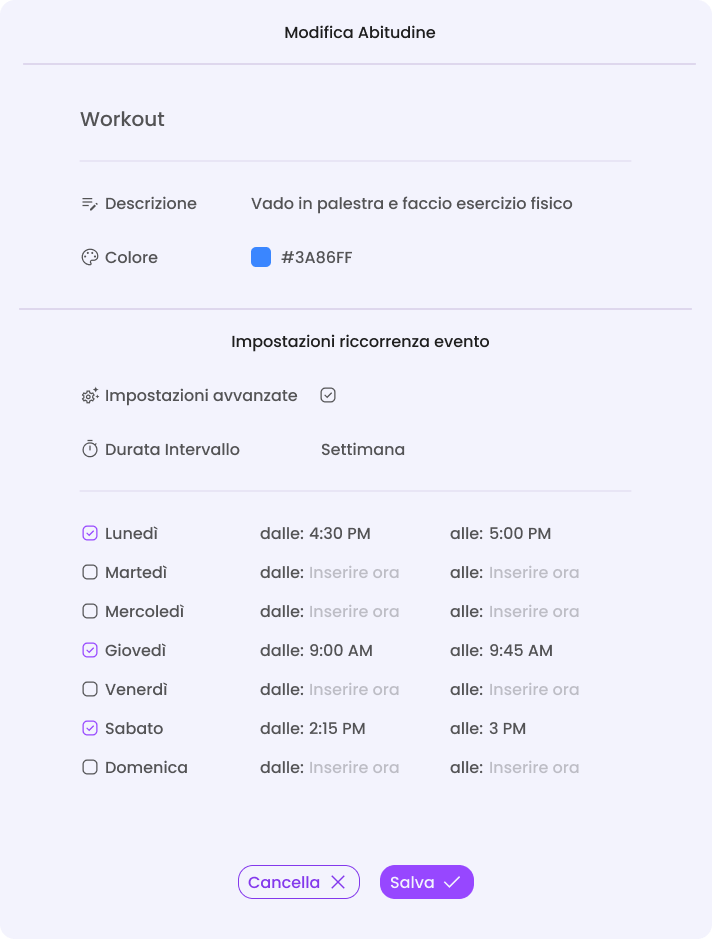
\includegraphics[width=0.49\textwidth,height=0.35\textheight]{img/FrontEnd/Abitudini/Modifica/ModificaAbitudineAvv.png}}
            \end{figure}
        \end{center}

    \end{listaPersonale2}
    \pagebreak
    \elemento [SCHERMATA ROUTINE] {fe:7} Nella schermata \href{https://www.figma.com/proto/cO66hx25OizBABGtWp8XlT/Planify?node-id=160%3A531&scaling=scale-down&page-id=0%3A1&starting-point-node-id=25%3A82}{“Routine”} l’utente ha possibilità di visualizzare e gestire tutte le proprie routine, ovvero le attività che ripete tutti i giorni (RF\ref{rf:5.5}), come dormire e mangiare. L’utente ha la possibilità di definire quante ore e quando avere queste attività di routine. L'utente può aggiungere le attività di routine da "Blocchi di attività" mediante un'azione di "drag and drop" nel tabella settimanale.
    \begin{figure}[H]
        \centering
        \href{https://www.figma.com/proto/cO66hx25OizBABGtWp8XlT/Planify?node-id=160%3A531&scaling=scale-down&page-id=0%3A1&starting-point-node-id=25%3A82}{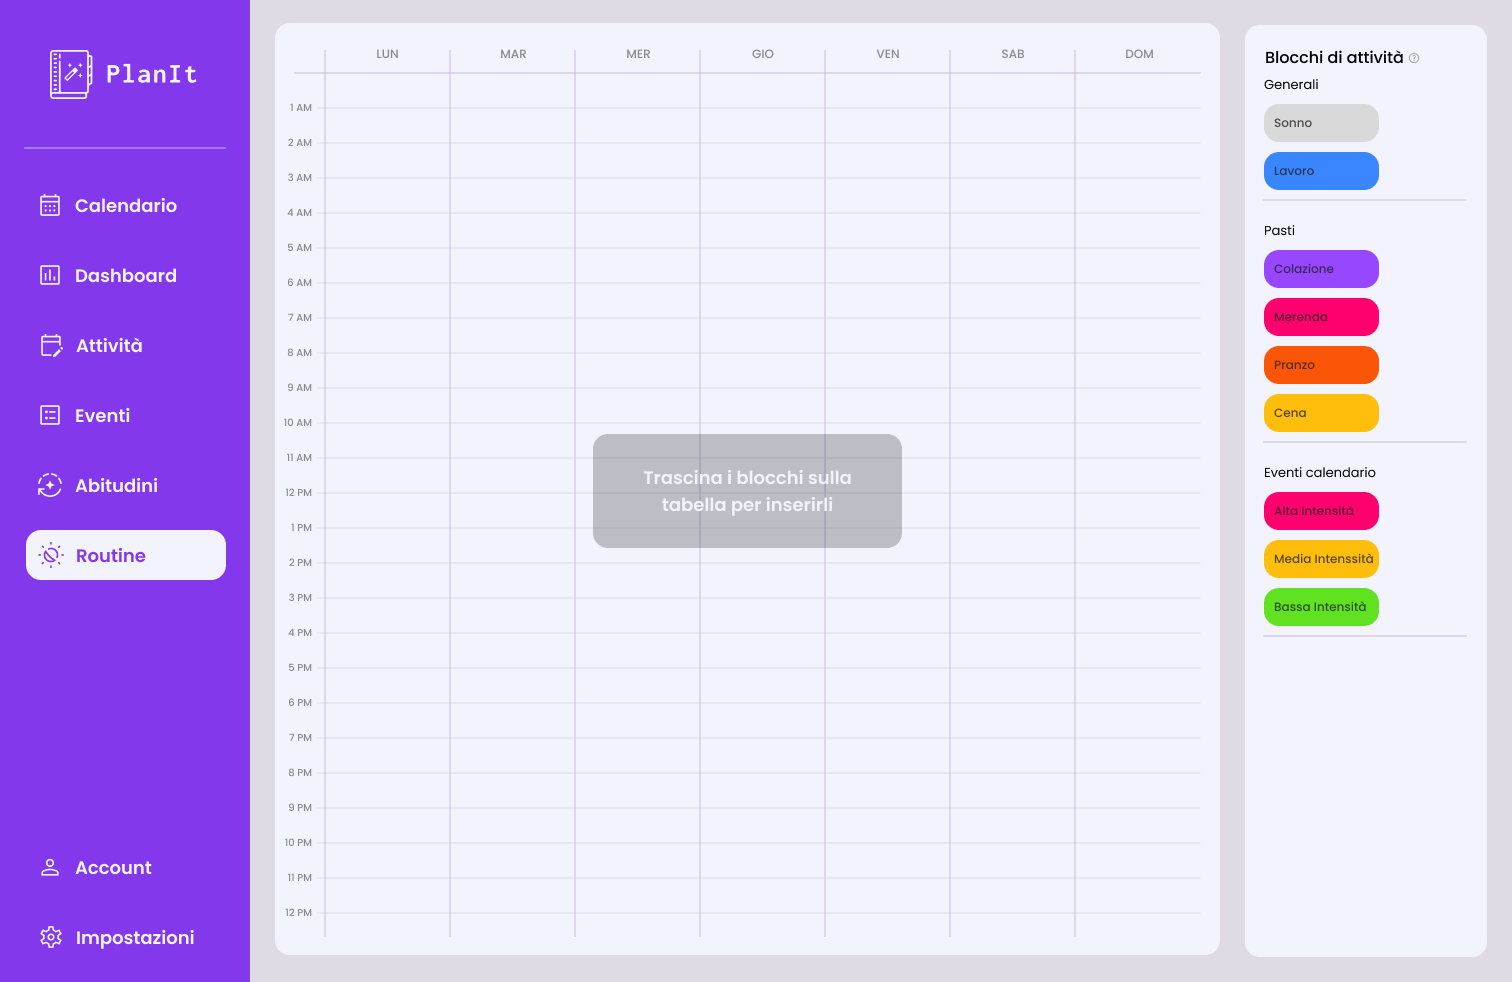
\includegraphics[width=1\textwidth]{img/FrontEnd/Routine/Routine.png}}
        \caption{Figura 7: schermata quando si apre la sezione "Routine"}
    \end{figure}
    \begin{figure}[H]
        \centering
        \href{https://www.figma.com/proto/cO66hx25OizBABGtWp8XlT/Planify?node-id=453%3A1711&scaling=scale-down&page-id=0%3A1&starting-point-node-id=25%3A82}{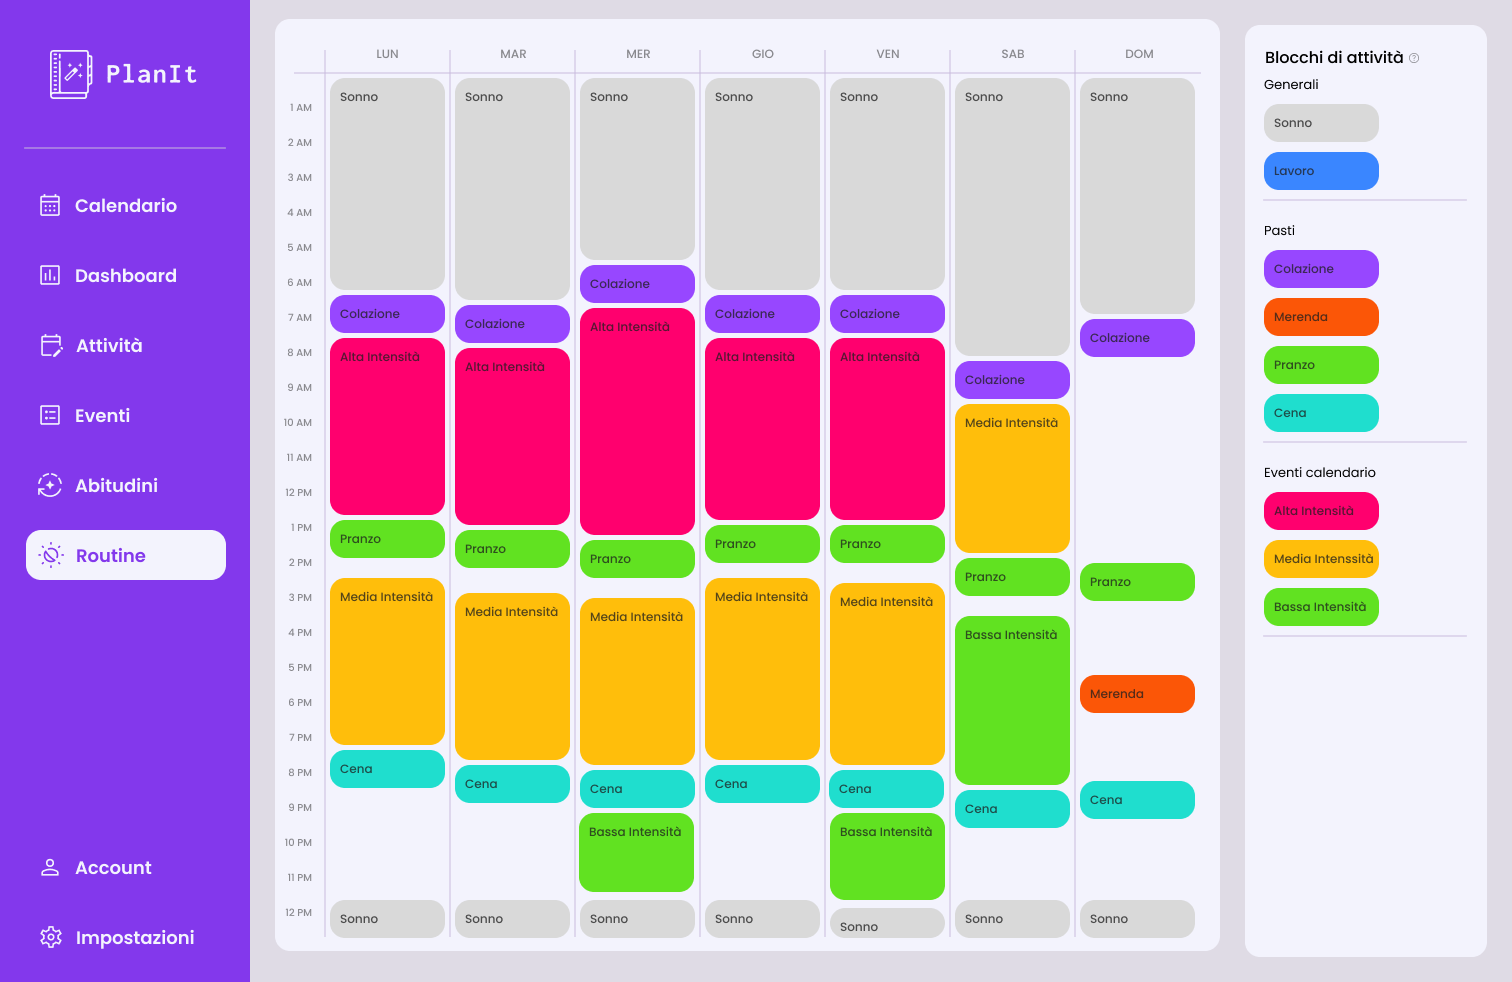
\includegraphics[width=1\textwidth]{img/FrontEnd/Routine/RoutineRiempito.png}}
        \caption{Figura 7.1: schermata quando si riempe il calendario settimanale con le routine mediante l'azione di "drag and drop"}
    \end{figure}
    

\end{listaPersonale}
\inclu{RequisitiBackEnd.tex}

Servizi usati
\begin{itemize}
    \item Googlle maps/OpenStreet maps
    \item Google calendar
    \item PayPal/Stripe
    \item Auth0
    \item Claudflare
\end{itemize}

\end{document}
